\documentclass[12pt]{report}
\usepackage[margin=2.5cm]{geometry}
\usepackage{amsmath, amssymb, amsthm}
\usepackage{physics}
\usepackage{float, subcaption, graphicx}
\usepackage{hyperref} % comment this in school template
\usepackage{setspace}
\synctex=1
\onehalfspacing

\theoremstyle{plain}
\newtheorem{proposition}{Proposition}

\theoremstyle{definition}
\newtheorem{definition}{Definition}

\newtheorem{theorem}{Theorem}

\newtheorem*{remark}{Remark}


\title{Instability of Flow In Magnetic Nozzle}
\author{Hunt Feng}

%%%%%%%%%%%%%%%%%%%%%%%%%%%%%%%%%%%%%%%%%%%%%%%%%%%%%%%%%%%%%%%%
% END OF FRONTMATTER SECTION
%%%%%%%%%%%%%%%%%%%%%%%%%%%%%%%%%%%%%%%%%%%%%%%%%%%%%%%%%%%%%%%%
\begin{document}
% Typeset the title page
\maketitle

\tableofcontents % remove this when using school template
% move abstract before the document in school template
\abstract{
    Spectral method is a common technique for analyzing the instability of a dynamical system. By discretizing the linearized equations motion of magnetic nozzle, the instability problem becomes a polynomial eigenvalue problem. Given Dirichlet boundary condition, we found that the flow with subsonic and supersonic velocity profiles are stable. Given fixed-open boundary condition, the subsonic flow is stable, but the supersonic flow is unstable. Different discretizations, such as finite difference, finite element and spectral element method agree with each other. By studying the convergence of different modes, we successfully eliminated the spurious unstable modes.

    However, spectral method is not enough to analyze the full problem. The problem has a singularity at the throat of the nozzle if the flow is transonic. The existence of singularity prevents the use of spectral method. We then expand the solution at the singularity and found the regular solution. Using that together with shooting method, we are able to solve the polynomial eigenvalue problem. The flow with accelerating velocity profile is stable.
}

%%%%%%%%%%%%%%%%%%%%%%%%%%%%%%%%%%%%%%%%%%%%%%%%%%%%%%%%%%%%%%%%
% FIRST CHAPTER OF THESIS BEGINS HERE
%%%%%%%%%%%%%%%%%%%%%%%%%%%%%%%%%%%%%%%%%%%%%%%%%%%%%%%%%%%%%%%%
\chapter{Introduction}
The title of this thesis involves several concepts, plasma, spectral instability, and magnetic nozzle. In the first chapter, we will introduce these concepts. Starting from the definition of plasma, then to the spectral instability and the general procedure of analyzing spectral instability. Following that, magnetic nozzle and magnetic mirror configuration will be introduced. After having these necessary knowledge, we are able to discuss the methods for analyzing the spectral instability of plasma flow in magnetic nozzle.

\section{Plasma}
Plasma is one of the fundamental states of matter, distinct from solid, liquid, and gas. In a plasma, the atoms or molecules have been stripped of electrons, resulting in a collection of charged particles, ions and electrons. In a vigorous sense, plasma is a fourth state of matter, though people often call it that way, because it does not involve phase transition. Plasma is the most common matter in the universe, it can be found in stars, including the sun, where nuclear fusion occurs at extremely high temperature. It also exists in solar wind, lightning and auroras. These natural plasmas can be seen in the sky because they are in plasma state, and plasma is capable of emitting light \cite{chen_introduction_2016}. Plasma has various scientific and technology uses. The artificially generated plasma can be found in fluorescent lights, Neon signs, etc. It can also be found in plasma physics research, nuclear fusion experiments, plasma cutting and welding, plasma medicine for treating diseases, and even in spacecraft propulsion systems. Overall, plasma is an intriguing and versatile state of matter with significant implications in various fields of science, technology, and industry. Fig.~\ref{fig:plasma-properties} lists some commonly seen natural and artificial plasmas.

\begin{figure}[htbp]
	\centering
	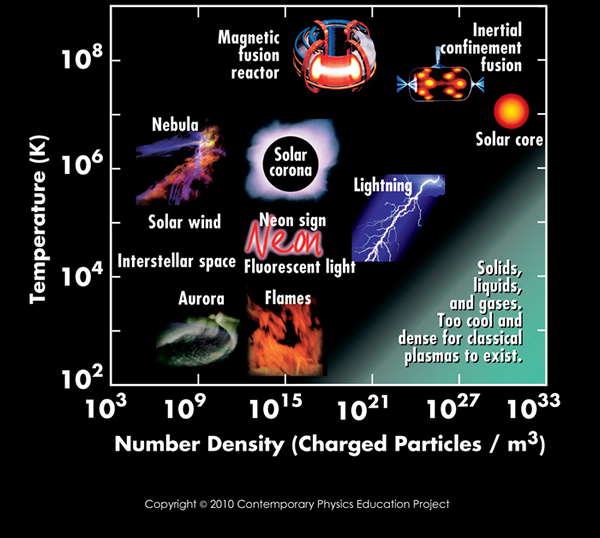
\includegraphics[width=0.7\textwidth]{figures/plasma-properties}
	\caption{Typical plasmas. Adapted from \cite{cpep_physics}.}
	\label{fig:plasma-properties}
\end{figure}

\subsection{Definition of Plasma}
In simple terms, a plasma is an ionized gas which is quasineutral and exhibits collective behavior \cite{chen_introduction_2016}. The following subsections will give precise definition of quasineutrality and collective behavior.

\subsubsection*{Debye Shielding and Quasineutrality}
A key characteristic of plasma is its capability to shield external electric field. Imagine a positively charged ball is put into a plasma (Fig.~\ref{fig:debye-shielding}, ions are neglected from the figure). Suppose there is sufficient amount of electrons in the plasma, and the plasma is cold, meaning that no thermal motions exist, the electric field generated by the ball will be shielded out by the surrounding electron cloud. If the plasma has finite temperature, then due to the thermal motions of electrons, the shielding will be incomplete and the edge of the electron cloud will be at the radius where potential energy is approximately equal to the thermal energy $KT$ \cite{chen_introduction_2016}.

\begin{figure}[htbp]
	\centering
	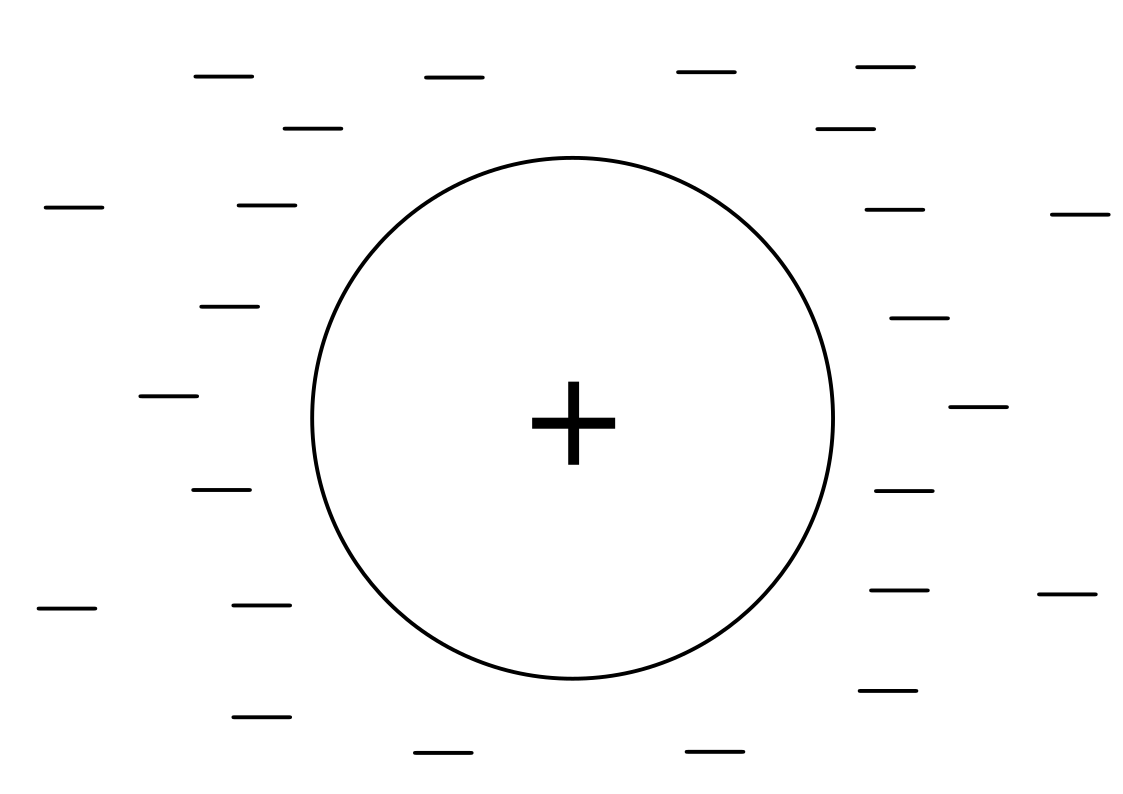
\includegraphics[width=0.4\textwidth]{figures/debye-shielding.png}
	\caption{Debye shielding. Adapted from \cite{chen_introduction_2016}. A positively charged ball is put into a plasma. Electrons will surround the ball. Ions are neglected from the picture since they are repelled away from the ball.}
	\label{fig:debye-shielding}
\end{figure}

The Debye length is the thickness of the electron cloud. To find out Debye length, we need to compute the potential near the positively charged ball. Due to the symmetry of the problem, we can reduce the it to 1D, along the radial direction. Suppose the coordinate's origin is at the ball's center and $\phi(0)=0$. The potential can be solved from the following 1-dimensional Poisson's equation,
\begin{equation}
	\epsilon_0\dv[2]{\phi}{x} = -e(n_i - n_e), \quad \phi(0) = \phi_0
	\label{eq:poisson-equation-1d}
\end{equation}
where $n$ is the number density of the particles, and the subscripts $i$ and $e$ stand for ion and electron.

For simplicity, we assume massless electron, $m/M \to 0$. This means that the electrons move so fast that the ions can be treated as a static background. That is,
\begin{equation}
	n_i = n_0
	\label{eq:ion-density-static-background}
\end{equation}
where $n_0$ is a constant.

Meanwhile, it can be proven using Fluid description of plasma that the electron density follows the Boltzmann distribution,
\begin{equation}
	n_e = n_0\exp(e\phi/KT_e)
\end{equation}

Taylor expand $n_e$ in the region where $\abs{e\phi/KT_e} \ll 1$ we have,
\begin{equation}
	n_e = n_0\left[ 1 + \frac{e\phi}{KT_e} + \frac{1}{2}\left(\frac{e\phi}{KT_e}\right)^2 + \cdots \right]
	\label{eq:electron-density-taylor-expansion}
\end{equation}

Substituting Eq.~(\ref{eq:ion-density-static-background}) and Eq.~(\ref{eq:electron-density-taylor-expansion}) for $n_i$ and $n_e$ in the 1D Poisson's equation, Eq.~(\ref{eq:poisson-equation-1d}), and only keep the linear terms in Eq.~(\ref{eq:electron-density-taylor-expansion}), we get
\begin{equation}
	\epsilon_0\dv[2]{\phi}{x} = \frac{n_0e^2}{KT_e}\phi
\end{equation}

The solution to the Poisson's equation is therefore,
\begin{equation}
	\phi = \phi_0\exp(-\abs{x}/\lambda_D)
\end{equation}
where the quantity $\lambda_D$ is called Debye length, and is defined as
\begin{equation}
	\lambda_D \equiv \left(\frac{\epsilon_0 KT}{ne^2}\right)^{1/2}
	\label{eq:debye-length}
\end{equation}
where $n$ stands for the number density far away from the charged ball. The potential is shown in Fig.~\ref{fig:debye-potential}. The  Debye length characterizes the thickness the of the cloud.

\begin{figure}[htbp]
	\centering
	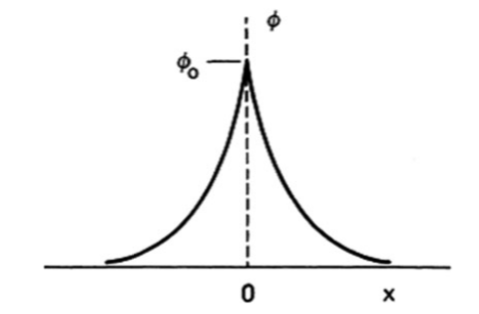
\includegraphics[width=0.7\textwidth]{figures/debye-potential.tikz}
	\caption{Potential distribution near a positively charged ball in a plasma. Adapted from \cite{chen_introduction_2016}. The charged ball is centered at the origin, the potential generated by this ball decreases exponentially.}
	\label{fig:debye-potential}
\end{figure}

The above discussion indicates that any external electric field present in a plasma will be shielded out within a distance $\lambda_D$ (assuming the system size $L$ is much larger than $\lambda_D$). Therefore, the plasma stays neutral if it is initially electrically neutral.

A plasma is said to be quasineutral, if a plasma is neutral enough so that we can take $n_i \simeq n_e$ but a small charge imbalance can give rise to potentials of the order of $KT/e$. In this case, we can the symbol $n$ to denote the common density and call it the plasma density \cite{chen_introduction_2016}.

\subsubsection*{Plasma Oscillation}
Simply speak, the collective behavior of a plasma is mostly governed by the electromagnetic forces rather than the gas dynamics. To quantify this statement, we introduce the concept of plasma oscillation.

There are many kinds of oscillations in plasma, one of the most fundamental oscillations is the electron plasma oscillation. Imagine the ions are too heavy to move, and they form a uniform background. The electrons are then released from a distance away from the ions (Fig.~\ref{fig:plasma-oscillation}). The electric field will pull the electrons toward the ions, after the electrons pass the ions, the electric field will decelerate them and started to pull them on the other side. The frequency of this oscillation is called plasma frequency,
\begin{equation}
	\omega_p = \left(\frac{n_0e^2}{\epsilon_0m}\right)^{1/2}
\end{equation}

\begin{figure}[htbp]
	\centering
	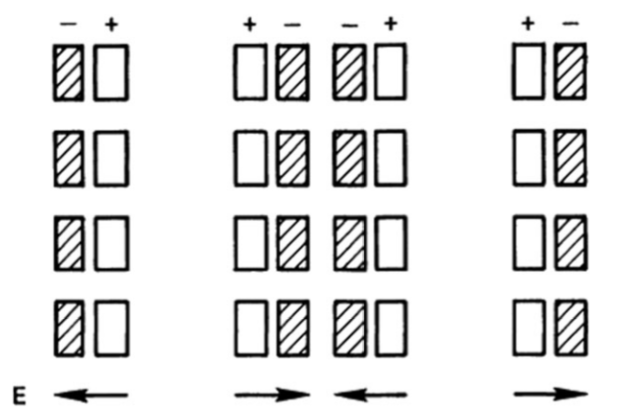
\includegraphics[width=0.7\textwidth]{figures/plasma-oscillation.tikz}
	\caption{Mechanism of plasma oscillations. Adapted from \cite{chen_introduction_2016}. As the electrons are pulled away from the ions, electric field forms and will pull the electrons back to the equilibrium position. Hence oscillation happens.}
	\label{fig:plasma-oscillation}
\end{figure}

\subsubsection*{Criteria of Plasma}
We are now able to give more detail definition for plasma. According to \cite{chen_introduction_2016}, not all ionized gas can be called plasma, there are three conditions a plasma must satisfy:
\begin{enumerate}
	\item Debye length is much smaller than the system size, $\lambda_D \ll L$.
	\item Collective behavior requires lots of particles in a Debye sphere, $N_D = n\frac{4\pi}{3}\lambda_D^3 \ggg 1$.
	\item The ionized gas behaves like plasma rather than a neutral gas, $\omega_p\tau > 1$ where $\omega_p$ typical plasma oscillation frequency and $\tau$ is the mean free time of collisions between neutral atoms.
\end{enumerate}


\section{Instability} \label{sec:instability-of-plasma-flow}
Magnetic nozzle is one of the most actively researched configurations in plasma propulsion systems, which is being developed for space missions due to their potential for high efficiency and thrust. Understanding and controlling instabilities in the plasma flow within these nozzles is essential for optimizing their performance and achieving efficient propulsion. Investigating instabilities in plasma flow within magnetic nozzles also contributes to our broader understanding of fundamental plasma physics phenomena. For instance, in astrophysics, the solar wind is accelerated by a magnetic mirror configuration similar to that of a magnetic nozzle, suggesting that our methodologies can also be applied to such problems.

\subsection{Plasma Instability}
The instability of plasma refers to the tendency of a plasma system to deviate from an equilibrium state under perturbations or fluctuations. It can be understood as the simple mechanical analogy with a ball on crest / in valley. On the left of Fig.~\ref{fig:stability-visualization} shows us a ball in its equilibrium and it is a stable equilibrium. Small perturbations given to the system will not push the ball far away from the equilibrium position, the valley. If friction exists, the ball oscillates with decreasing amplitude and will eventually reached the equilibrium state as time goes to infinity. Hence, the equilibrium is stable. On the right, any small perturbations will cause the ball to fall downhill and will never come back to the initial equilibrium position. Hence this equilibrium is unstable.

\begin{figure}[htbp]
	\centering
	\begin{subfigure}[b]{0.5\textwidth}
		\centering
		\includegraphics[width=0.7\linewidth]{figures/stability-visualization-stable.tikz}
		\caption{Stable equilibrium.}
	\end{subfigure}%
	\begin{subfigure}[b]{0.5\textwidth}
		\centering
		\includegraphics[width=0.7\linewidth]{figures/stability-visualization-unstable.tikz}
		\caption{Unstable equilibrium.}
	\end{subfigure}
	\caption{Mechanical analogy of various types of equilibrium. Adapted from \cite{chen_introduction_2016}.}
	\label{fig:stability-visualization}
\end{figure}


The instabilities in plasma can arise from various factors, such as the interaction of particles with electromagnetic fields, collective effects, or the presence of gradients in plasma parameters. A famous example of instability is the two stream instability. The configuration starts with two oppositely traveling beams of ions and electrons. As time evolves, the two beams can no longer stay in its equilibrium state due to the electromagnetic interactions, and chaotic behavior develops as shown in Fig.~\ref{fig:two-stream-instability}.

\begin{figure}[htbp]
	\centering
	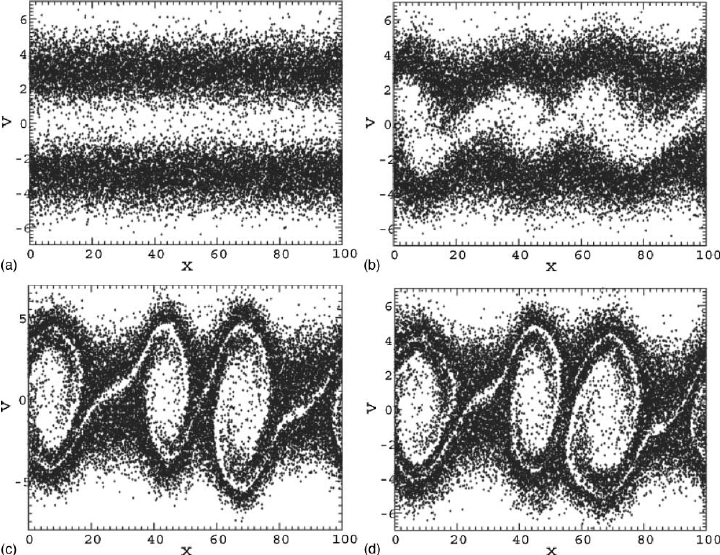
\includegraphics[width=0.7\linewidth]{figures/two-stream-instability}
	\caption{Visualization of two-stream instability in the phase space. (a) Initially the ion and electron flow are in opposite direction. (b) The velocity of both flows start to oscillate. (c) Chaotic behavior occurs. (d) The chaotic behavior continues. Adapted from \cite{ha_nonlinear_2011}.}
	\label{fig:two-stream-instability}
\end{figure}

\subsection{Spectral Instability of Partial Differential Equations}
In the study of partial differential equations (PDEs), there are two types of instability: structural instability and dynamic instability. The structural instability refers to the tendency of the solution to diverge under perturbations in the PDE parameters, while the dynamic instability refers to the tendency of solution to deviate from a stationary solution given perturbations in the stationary solution \cite{beck_spectral_2020}. We are interested in the dynamic instability. In this subsection, we will describe the process for investigating plasma instability, and explain why we can investigate the dynamic instability by analyzing the spectrum of the linear operator of the corresponding linearized PDE. Hence the name spectral instability. We will discuss the connection between spectral instability and the plasma instability later in this subsection.

In order to investigate the plasma instability, the first step is to state the governing equations for the plasma flow in the magnetic nozzle. The governing equations are time-dependent fluid equations involving the number density $n$ and fluid velocity $v$ of the plasma flow along the central axis of the nozzle,
\begin{equation}
	\pdv{t}\mqty[n\\ v] + \mathbf{F}(n,v) = \mathbf{0}
	\label{eq:pde-system}
\end{equation}
This PDE system has two first-order PDEs, Eq.~(\ref{eq:conservation-of-density}) and Eq.~(\ref{eq:conservation-of-momentum}). Detail derivation will be given in Sec.~\ref{sec:equation-of-motion-of-the-plasma-flow-in-nozzle}.

Following this we find the equilibrium state (stationary solution) to the above PDE system, Eq.~(\ref{eq:pde-system}). In other words, we find $n_0$ and $v_0$ such that $\mathbf{F}(n_0,v_0)=\mathbf{0}$. The expression of equilibrium velocity $v_0$ is given by Eq.~(\ref{eq:velocity-profile}) and it can be found in Sec.~\ref{sec:velocity-profiles}. The details of derivation and Lambert-W will be explained in Sec.~\ref{sec:velocity-profiles}. As for $n_0$, it is not required to obtain its expression because we are able to reduce the linearized first-order PDE system Eq.~(\ref{eq:pde-system}) into a second-order PDE by eliminating the density $n$.

Now we are in a stage ready to investigate the dynamic instability of the problem. The system will be given small spatial perturbations, they serve as small fluctuations on number density and velocity, $\tilde{n}(z)$ and $\tilde{v}(z)$. All variables $n$ and $v$ in the governing equations will be substituted by perturbed quantities, $n_0+\tilde{n}$ and $v_0+\tilde{v}$. The PDE system Eq.~(\ref{eq:pde-system}) now becomes,
\begin{equation}
	\underbrace{\pdv{t}\mqty[\tilde{n}\\ \tilde{v}] + d\mathbf{F}(n_0,v_0)\mqty[\tilde{n}\\ \tilde{v}] }_{linear terms}
	+ \underbrace{\mathbf{F}(n_0+\tilde{n}, v_0+\tilde{v}) - d\mathbf{F}(n_0,v_0)\mqty[\tilde{n}\\ \tilde{v}]}_{non-linear terms}
	= \mathbf{0}
	\label{eq:perturbed-pde-system}
\end{equation}

Since $\tilde{n}$ and $\tilde{v}$ are small, we expect the higher order mixed terms such as $\tilde{n}\tilde{v}$, $\tilde{n}\partial_z\tilde{v}$, $\tilde{v}\partial_z\tilde{n}$ are negligible comparing to the linear terms. So we drop the non-linear terms. Now we obtain the so-called linearized governing equations, they are the linearized conservation of density, Eq.~(\ref{eq:linearized-conservation-of-density}) and the linearized conservation of momentum, Eq.~(\ref{eq:linearized-conservation-of-momentum}), respectively.

Since we are dealing with linear operators, let the perturbations take the form of exponential $\exp(-i\omega t)$. This indicates that physically the perturbations are oscillating with frequency $\omega$ in time. Any time derivative on the perturbations in the linearized governing equations simply becomes $\partial_t \to -i\omega$. Now we obtain equations involving perturbations, $\tilde{n}$ and $\tilde{v}$, and their spatial derivatives, and $\omega$. Reducing the number of equations by eliminating the density $\tilde{n}$, we obtain Eq.~(\ref{eq:polynomial-eigenvalue-problem}).

The problem of investigating the plasma instability becomes the problem of finding the eigenvalues, $\omega$, of Eq.~(\ref{eq:polynomial-eigenvalue-problem}) under different boundary conditions. The connection between the eigenvalue $\omega$ and the plasma instability is clear: The oscillation frequency $\omega$ is a complex number. If the imaginary part of the temporal frequency is greater than zero, i.e. $\Im(\omega) > 0$, then the system is unstable. This is because the perturbation grows exponentially $\exp(\Im(\omega)t)$ in time. On the other hand, if the imaginary part of the temporal frequency is less than or equal to zero, $\Im(\omega) \leq 0$, then the system is said to be stable. Since the perturbations will not be growing, $\Im(\omega)=0$, or even damped, $\Im(\omega) < 0$.

Since the PDE we analyze is linear, its spectral instability is also called linear instability. In this following thesis, the terms plasma instability, spectral instability, linear instability will be used interchangeably, sometimes an even shorter term instability will be used.

We will devote the rest of the chapters to develop methods for solving the eigenvalue problem Eq.~(\ref{eq:polynomial-eigenvalue-problem}). We will employ spectral methods to obtain eigenvalues for subsonic and supersonic velocity profiles, and shooting method will be used to get eigenvalues when velocity profile $v_0$ is accelerating.

\section{Magnetic Nozzle}
In this thesis, we are going to deal with plasma flow in magnetic nozzle.
A magnetic nozzle is a device that uses a magnetic field to shape and control the flow of charged particles in a plasma propulsion system, see Fig.~\ref{fig:magnetic-nozzle}. By employing magnetic mirrors, the magnetic nozzle can efficiently direct and accelerate the plasma particles, generating thrust for propulsion. The magnetic field in the nozzle helps collimate and focus the plasma exhaust, increasing its velocity and enhancing the performance of the propulsion system.

\begin{figure}[htbp]
	\centering
	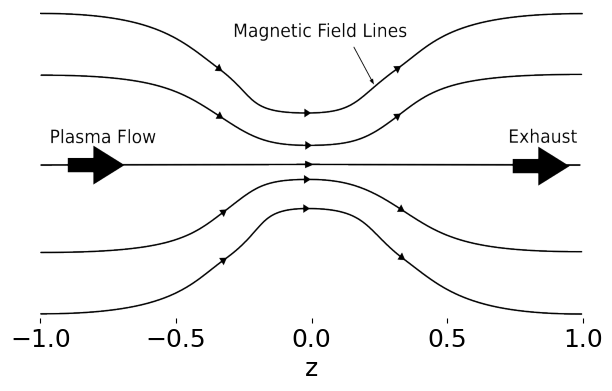
\includegraphics[width=0.7\linewidth]{figures/magnetic-nozzle.png}
	\caption{A simplified example of a magnetic nozzle configuration. On the left ($z=-1$) is the entrance of the nozzle. The plasma flows into the nozzle from the left and will be accelerated and finally exhaust through the exit on the right ($z=1$). The magnetic field lines are shaped in such a way that it forms a magnetic mirror configuration. Plasma flow with specific subsonic speed at the entrance will be accelerated to supersonic speed.}
	\label{fig:magnetic-nozzle}
\end{figure}

\subsection{Magnetic Field in Magnetic Nozzle} \label{sec:magnetic-field-in-nozzle}
The magnetic nozzle by its nature is 3-dimensional. We assume the magnetic field is axis-symmetric, then the radial magnetic field and axial magnetic field are constraint by divergence-free condition,
\begin{equation}
	\div\mathbf{B} = \frac{1}{r}\pdv{(rB_r)}{r} + \pdv{B_z}{z} = 0
	\label{eq:divergence-free-condition}
\end{equation}
Since we are interested in the plasma flow near the central axis of the nozzle, with paraxial approximation taken, the derivative along the magnetic field line $\nabla_\parallel = \pdv*{z}$ when near the central axis \cite{smolyakov_quasineutral_2021}. Hence, in this thesis we will treat the flow in magnetic nozzle as a 1-dimensional problem. The axial magnetic field along the central axis is modeled as
\begin{equation}
	B_z(z) = B_0 \left[1 + R\exp(-\left(\frac{z}{\delta}\right)^2)\right], \quad -1\leq z \leq 1
\end{equation}
where $1+R$ is the magnetic mirror ratio, it is the ratio of the magnitude of magnetic field at the center of the nozzle to that at the end of the nozzle, $1+R = B(0)/B(1)$. The mirror ratio $R$ controls the spread of the plasma flow at the exit. On the other hand, $\delta$ determines the spread of the magnetic field. Larger the $\delta$, flatter the magnetic field. An example of magnetic field is shown in Fig.~(\ref{fig:magnetic-field}).

The radial profile of magnetic field, $B_r$, is given by the divergence-free condition, Eq.~(\ref{eq:divergence-free-condition}). In this thesis will focus on the axial magnetic field only.

\begin{figure}[htbp]
	\centering
	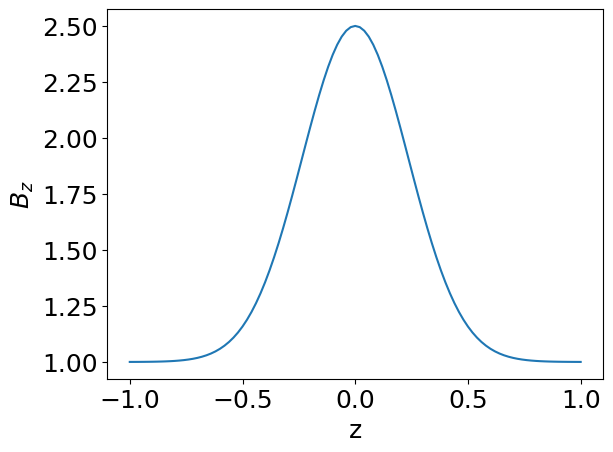
\includegraphics[width=0.7\linewidth]{figures/magnetic-field}
	\caption{This is the magnetic field in nozzle with mirror ratio $1+R=B_{max}/B_{min}=2.5$, and the spread of magnetic field, $\delta=0.1/0.3=0.\bar{3}$. }
	\label{fig:magnetic-field}
\end{figure}

\subsection{Velocity Profiles of Plasma Flow in Magnetic Nozzle}
The analytical solution gives 4 different kinds of velocity profiles,
\begin{itemize}
	\item Subsonic profile: Plasma flow enters and exits the nozzle with subsonic speed. Every point on this profile is subsonic.
	\item Supersonic profile: Plasma flow enters and exits the nozzle with supersonic speed. Every point on this profile is supersonic.
	\item Accelerating profile: Plasma flow enters the nozzle with subsonic speed and exits the nozzle with supersonic speed. Points before the nozzle throat are subsonic, and the flow reaches ion sound speed at the nozzle throat, then the flow is supersonic after the nozzle throat.
	\item Decelerating profile: Plasma flow enters the nozzle with supersonic speed and exits the nozzle with subsonic speed. Similar to the accelerating profile, but the velocity is decreasing.
\end{itemize}
See Fig.~\ref{fig:velocity-profiles} for these profiles.

The velocity of plasma flow in the magnetic nozzle is given by the Lambert W function, Eq.~(\ref{eq:velocity-profile}). The Lambert W function has 2 different branches. The $k=0$ branch corresponds to the subsonic parts in the velocity profile, and the $k=-1$ branch gives the supersonic parts. The expression of velocity profile will be derived in Chap.~\ref{chap:polynomial-eigenvalue-problem} and more details will be discussed.

\section{Flow in Similar Configuration: Bondi-Parker Flow}
Consider a massive celestial object in the space. This celestial object will attract matter in the space because it is massive. Hence, creating an accretion flow. If the celestial object is a star, it can also eject matter into space. Solar wind is an example to this since it is a stream of charged particles, primarily electrons and protons, flowing outward from the Sun. Bondi derived a steady-state solution for accretion flow which is governed by Bernoulli's equation in spherical symmetry around a point mass in 1952. Hence, the inward accretion flow is also called Bondi flow. Then Parker solved a similar problem but with outward wind in 1958. Then the outward wind is given the name, Parker flow \cite{aikawa_stability_1979,bondi_spherically_1952,keto_stability_2020}. The Bondi and Parker flow (also called Bondi-Parker flow) is similar to that in magnetic nozzle. It is interesting to compare the two configurations.

If we compare the velocity profiles for Bondi-Parker flow and the flow in magnetic nozzle. We found they are similar. The Bondi-Parker flow can also be grouped into the following types: subsonic, supersonic, and transonic (accelerating and decelerating). See Fig.~\ref{fig:BP-flow-velocity}. For subsonic profiles, every point on the curve is slower than sound speed. While every point on the supersonic velocity profile is faster than sound speed. Lastly, there are two different transonic profiles: accelerating profile and decelerating profile. The accelerating profile describes the accelerating plasma flow which is at subsonic speed at the mass point, e.g. a star, and is accelerated to supersonic speed far away. The decelerating profile shows that a plasma flow ejected supersonically from a mass point and then decelerated to subsonic speed far away.

The velocity profiles of one-dimensional, spherically symmetric, stationary isothermal Parker flow neglecting self-gravity can be expressed using Lambert W function,
\begin{equation}
	v(r) = \sqrt{-\frac{KT}{m}W_k\left[ -\left(\frac{r}{r_c}\right)^2 \exp\left[4\left(1-\frac{r_c}{r}\right)-1\right] \right]}, \quad
	k = 0,-1
\end{equation}
where $r$ stands for the distance measured from the center of the mass point, e.g. star. The position $r_c=GMm/2KT$ is the critical position and the velocity at this point is exactly the sonic speed $v(r_c)=\sqrt{KT/m}$, where $M$ is the mass of the mass point, $m$ is the mass of a single particle in the flow, and $T$ is the temperature of the flow. The Bondi flow is simply $-v(r)$ since it is accretion flow, the particles are flowing inwardly towards the mass point.

As we can see the expression of velocity profile for Bondi-Parker flow is similar to that of the magnetic nozzle, Eq.~(\ref{eq:velocity-profile}). The expression is governed by the Lambert W function. Similarly, the $k=0$ branch corresponds to the subsonic part in the velocity profile, and the $k=-1$ branch corresponds to the supersonic part of the profile.

\begin{figure}[htbp]
	\centering
	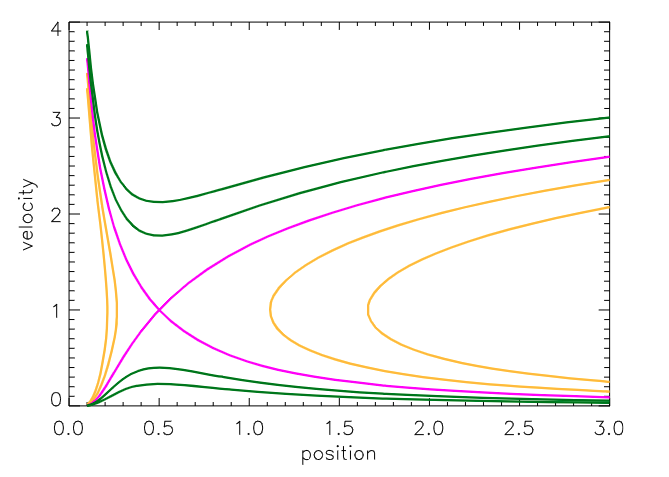
\includegraphics[width=0.7\textwidth]{figures/steady-state-BP-flow}
	\caption{Representative trajectories of the steady-state BP flow in non-dimensional units. The velocities are shown in absolute values. Adapted from \cite{keto_stability_2020}. The upward pink line represents an accelerating flow, it accelerates from subsonic to supersonic. The downward pink line represents a decelerating flow. The green lines below the pink lines represent subsonic flows, and the green lines above represent supersonic flows. Orange lines are physically impossible scenarios. If the sign of the velocity is positive, then it is an outward (Parker) flow, otherwise it is an inward (Bondi) flow.}
	\label{fig:BP-flow-velocity}
\end{figure}

The instabilities of the Bondi-Parker flow has been extensively studied \cite{bondi_spherically_1952,velli_from_1994,velli_hydrodynamics_2001,del_dynamical_1998,keto_stability_2020}. Hopefully these studies can provide insights into our problem.

\section{Goals of this Thesis}
Fusion is considered the next-generation source of a clean, safe and abundant energy providing an opportunity to address climate change problems. A new high-tech industry has appeared in the last decade fueled by over \$4 billion of private investments, with the second world largest and several other smaller companies founded in Canada. To achieve controlled fusion, one of the key science problems is to understand and learn to predict the non-linear behavior of plasma due to waves and instabilities. The general objective of my research is to understand the behavior and learn to control the turbulent flows of plasmas in magnetically controlled fusion system, in particular, open magnetic mirrors. I study the instabilities of the flow in a magnetic mirror configuration under different boundary conditions which is an open question and is under debate in application to fusion systems and also related to the solar wind flows.

The general objective of this research is to understand the stability of the flow in a magnetic nozzle. Plasma confined by the magnetic field is typically far from the state of the thermodynamic equilibrium which makes it unstable. In this project, we would like to investigate the stability of plasma flow in a magnetic nozzle under different boundary conditions. Understanding the instabilities of plasma flow in a magnetic mirror configuration is important in applications such as the expanding magnetic divertors in controlled fusion and electric propulsion \cite{ryutov_divertor_2016,kaganovich_2020_physics}.

In the following thesis, fluid model of plasma will be reviewed and linearized governing equations will be derived in chapter \ref{chap:polynomial-eigenvalue-problem}. The problem will be then formulated as an eigenvalue problem. In chapter \ref{chap:spectral-method}, spectral method for solving eigenvalue problem will be introduced. Spectral-collocation and spectral-Galerkin methods will be discussed. Moreover, spectral pollution and the filtering techniques will as also be investigated. If the velocity profile is transonic, the existence of singularity at the nozzle throat prevents the use the spectral methods, therefore we will formulate the problem to the form suitable for applying shooting method. In chapter \ref{chap:singular-perturbation} we will discuss the existence of the singularity and then extract the regular solutions using Frobenius method. After this, we will apply shooting method to the problem and investigate the instabilities. Conclusion will in chapter \ref{chap:discussion}.

\chapter{Theoretical Analysis} \label{chap:theoretical-analysis}
In this chapter, we first examine the single particle motion along the magnetic field, subsequently to a kinetic description of plasma. Following this, we derive the fluid description of plasma. After this, we establish the governing equations for flow in the magnetic nozzle. Following their derivation, we proceed to linearize these governing equations and reframe the problem as a polynomial eigenvalue problem. Finally, we analytically explore a special case.

\section{Kinetic Theory}
\subsection{Single Particle Motion in Uniform Magnetic and Electric Fields} \label{sec:single-particle-motion}
Plasma consists of charged particles, and is governed by electromagnetic force. This subsection gives a description of single particle motion with the presence of uniform magnetic and electric fields. This gives us intuition of how the particles move in a magnetic nozzle. Since the particle motion is governed by Lorentz force, the equation of motion of a charged particle is given by
\begin{equation}
	m\dv{\mathbf{v}_p}{t} = q(\mathbf{E} + \mathbf{v}_p\times \mathbf{B})
	\label{eq:equation-of-motion-single-particle}
\end{equation}
where $m$ is the mass of charged particle, $q$ is its electric charge, and $\mathbf{v}_p$ is the particle's velocity.

\subsubsection*{No Electric Field}
Consider a uniform magnetic field pointing in z-direction, $\mathbf{B}=B\mathbf{\hat{z}}$, and no electric field for now. Since the magnetic force is perpendicular to both $\mathbf{v}_p$ and $\mathbf{B}$, we can separate the equation of motion into two directions,
\begin{equation}
	\begin{aligned}
		m\dv{\mathbf{v_\parallel}}{t} & = \mathbf{0}                 \\
		m\dv{\mathbf{v_\perp}}{t}     & = q\mathbf{v_\perp \times B}
	\end{aligned}
\end{equation}
where $\mathbf{v_\parallel}$ denotes the velocity along the magnetic field line, in this case $v_\parallel = v_z$, and $\mathbf{v_\perp}$ is the velocity perpendicular to the magnetic field, in this case $\mathbf{v_\perp} = v_x\hat{x} + v_y\hat{y}$. Solving these equations with initial condition $\mathbf{v_p}|_{t=0} = v_{0x}\hat{x} + v_{0y}\hat{y} + v_{0z}\hat{z}$  we get
\begin{equation}
	\begin{aligned}
		v_x & = v_{0\perp} e^{i\omega_c t}      \\
		v_y & = \pm iv_{0\perp} e^{i\omega_c t} \\
		v_z & = v_{0z}
	\end{aligned}
\end{equation}
where $v_{0\perp} = \sqrt{v_{0x}^2+v_{0y}^2}$ is the initial speed in the plane perpendicular to the magnetic field, and $\omega_c \equiv \abs{q}B/m$ is called the Larmor frequency. In this way, we see that the charged particle is doing circular motion in the $x-y$ plane with Larmor frequency $\omega_c$. On the other hand, the particle is flowing freely in $\hat{z}$ direction since there is no force acting on the charged particle along the magnetic field line. The charged particle is doing helical motion along the magnetic field line. See Fig.~\ref{fig:gyrate-along-b-field}. If we integrate the velocities with respect to time we will see the radius of the gyration is a constant, $r_L \equiv m_v\perp/\abs{q}B$, it is called Larmor radius.

\subsubsection*{Finite Electric Field}
With the presence of uniform electric field $\mathbf{E} = E_x\hat{x} + E_y\hat{y} + E_z\hat{z}$, the solution to Eq.~(\ref{eq:equation-of-motion-single-particle}) becomes

\begin{equation}
	\begin{aligned}
		v_x & = v_{0\perp} e^{i\omega_c t} + \frac{E_y}{B}      \\
		v_y & = \pm iv_{0\perp} e^{i\omega_c t} - \frac{E_x}{B} \\
		v_z & = v_{0z} + \frac{qE_z}{m}t
	\end{aligned}
\end{equation}
In the direction along the magnetic field, electrostatic force is acting on the particle causing it to accelerate / decelerate with constant acceleration $qE_z/m$. In the direction perpendicular to magnetic field, the Larmor radius is still $r_L = m_v\perp/\abs{q}B$ but the particle's guiding center drifts with velocity
\begin{equation}
	\mathbf{v_{E\times B}} = \frac{\mathbf{E\times B}}{B^2} = \frac{E_y}{B}\hat{x} - \frac{E_x}{B}\hat{y}
\end{equation}
This is so-called the $\mathbf{E\times B}$ drift.

Imagine a cylinder shape magnetic nozzle with externally applied magnetic field, the magnetic field is as described in Sec.~\ref{sec:magnetic-field-in-nozzle}. The particles will move along the magnetic field lines. Due to high mobility of electrons, they move faster than ions, this creates electric field and will accelerate ions in the nozzle (more details will be discussed in Sec.~\ref{sec:equation-of-motion-of-the-plasma-flow-in-nozzle}). By symmetry, if there is electric field in the plane perpendicular to $\mathbf{B}$ field, it will be pointing radially, $\mathbf{E_\perp} = E_\perp\cos\theta\hat{x} + E_\perp\sin\theta\hat{y}$. According to the above discussion, the $\mathbf{E\times B}$ drift, $\mathbf{v_{E\times B}} = E_\perp/B (\sin\theta\hat{x} - \cos\theta\hat{y})$, will be in $\hat{\theta}$ direction. Meaning that in magnetic nozzle, the particles have two gyrating motions: one is the small scale Larmor gyration, and the other one is the larger scale $\mathbf{E\times B}$ drift in $\hat{\theta}$ direction. In this thesis, we are interested in the flow near the central axis, therefore the larger scale drift will be ignored.

\subsection{Adiabatic Invariants}
The charged particles always travel on the same magnetic field line in the magnetic nozzle. To show this we will introduce two adiabatic invariants.

\subsubsection*{Magnetic Moment}
In classical mechanics, the action integral $\oint pdq$ taken over a period of a periodic motion is a constant. Here $p$ and $q$ are generalized momentum and coordinate. In single particle motion along magnetic field line, one obvious periodic motion is the Larmor gyration. Take $p$ to be the angular momentum $mv_\perp r$ and $q$ to be the angular coordinate $\theta$, the action integral becomes

\begin{equation}
	\oint pdq = \oint mv_\perp r_L d\theta = 2\pi r_L mv_\perp = 2\pi \frac{mv_\perp^2}{\omega_c} = 4\pi\frac{m}{\abs{q}}\left(\frac{mv_\perp^2}{2B}\right)
\end{equation}

Define the quantity magnetic moment as

\begin{equation}
	\mu = \frac{mv_\perp^2}{2B}
\end{equation}

We see that the magnetic moment $\mu$ is constant as long as $q/m$ is constant.

\subsubsection*{Longitudinal Invariant}
The next adiabatic invariant is the quantity defined as \cite{chen_introduction_2016}
\begin{equation}
	J=\int_a^b v_\parallel ds
\end{equation}
where $a$ and $b$ are the two turning points in magnetic mirror, see Fig.~\ref{fig:particle-in-mirror}.

\begin{figure}[htbp]
	\centering
	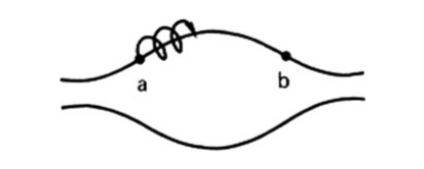
\includegraphics[width=0.7\textwidth]{figures/particle-in-mirror.png}
	\caption{A particle bouncing between turning points $a$ and $b$ in a magnetic field. Adapted from \cite{chen_introduction_2016}.}
	\label{fig:particle-in-mirror}
\end{figure}

Since the particle's energy is conserved and is equal to $mv_\perp^2/2$ at the turning point, the invariance of $\mu$ indicates that $\abs{B}$ remains the same at the turning point. However, upon drifting back to the same longitude, a particle may find itself on another line of force at a different altitude. This cannot happen if $J$ is conserved. $J$ determines the length of the line of force between turning points, and no two lines have the same length between points with the same $\abs{B}$. Consequently, the particle returns to the same line of force even in a slightly asymmetric field.


\begin{figure}[htbp]
	\centering
	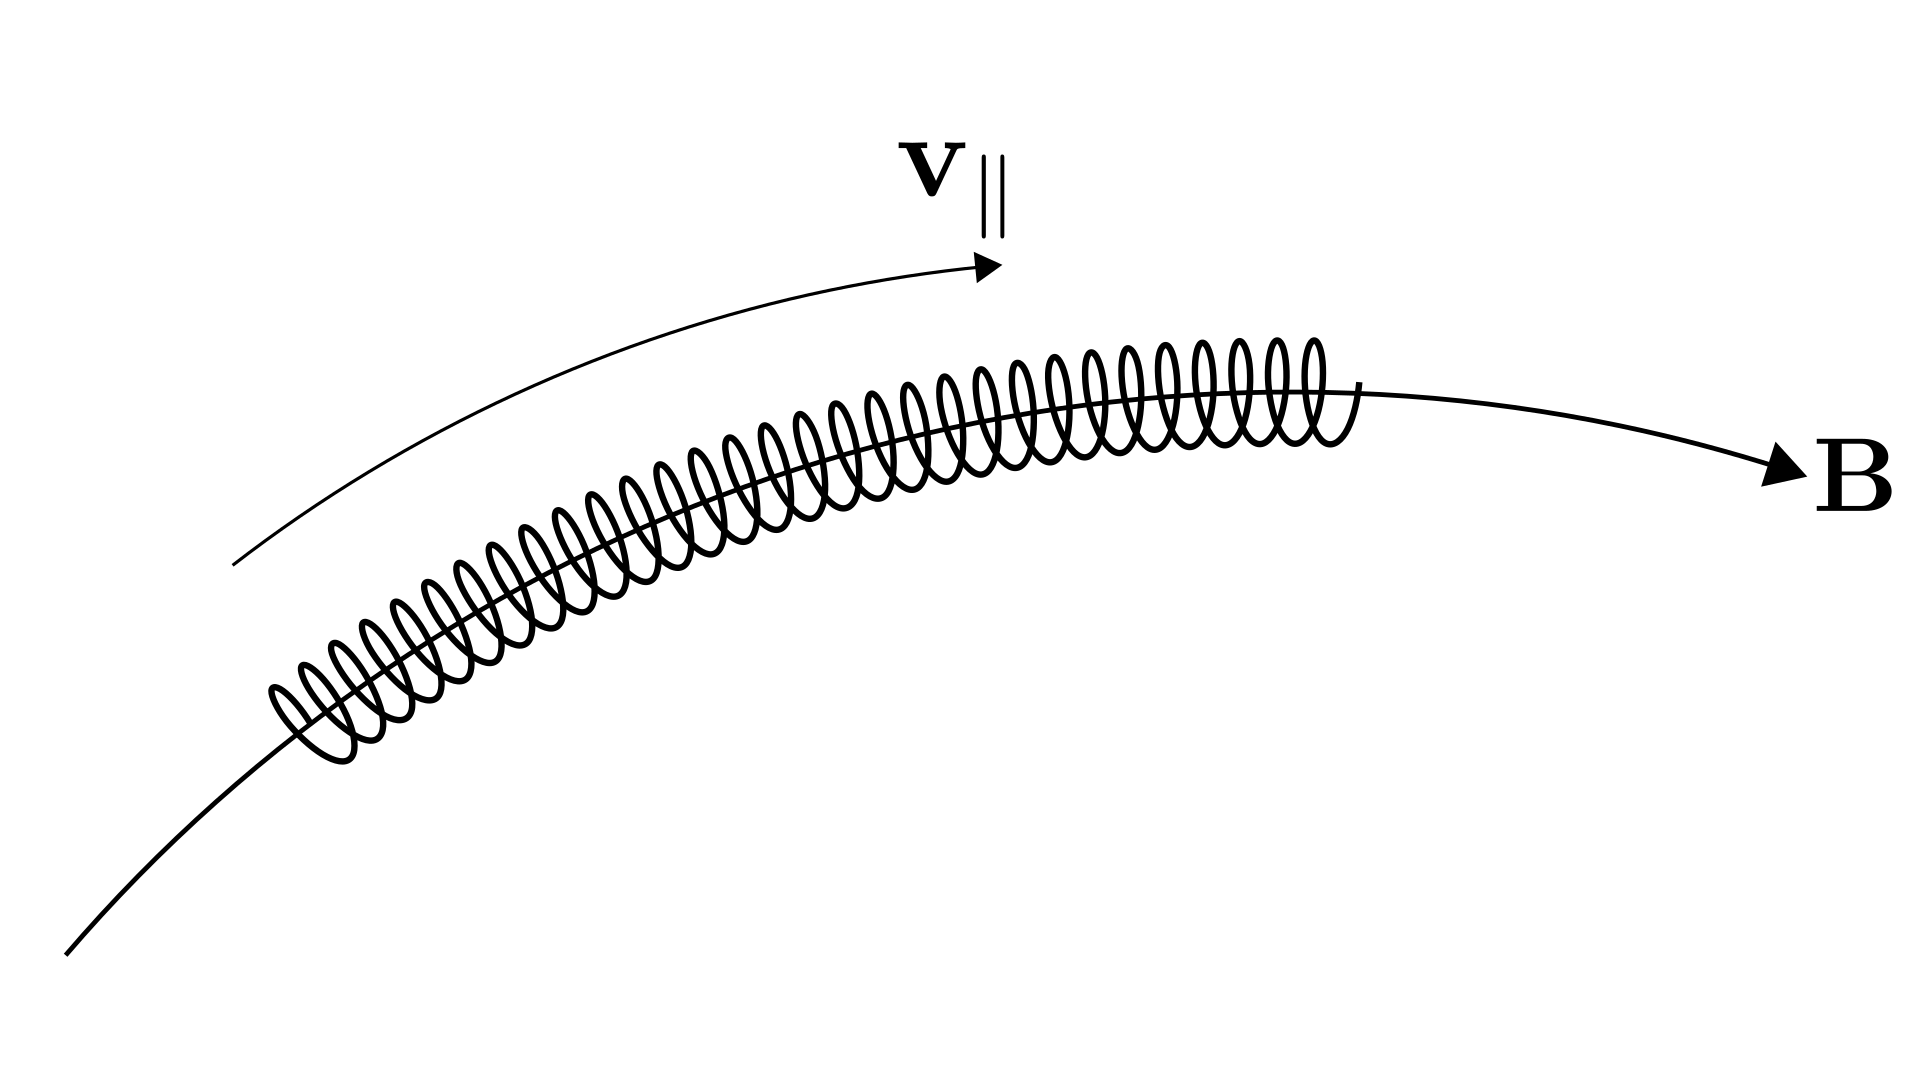
\includegraphics[width=0.7\linewidth]{figures/gyrate-along-b-field}
	\caption{A charged particle gyrates about the magnetic field line. The velocity along the field line is $\mathbf{v}_{\parallel}$ and the gyrate frequency, radius is given by the radial equation, $q\mathbf{v_{\perp}\times B} = \mathbf{\hat{r}} mv_\perp^2/r$. Moreover, for static, nonuniform magnetic field, the charged particle will stay on the same of magnetic field line as it gyrates.}
	\label{fig:gyrate-along-b-field}
\end{figure}

\subsection{From Kinetic Theory to Fluid Description}
Although the previous treatment is useful for single particle, to describe the collective behavior of a large amount of particles, we need to do that in the framework of kinetic theory. In kinetic theory, the charged particles in plasma obey a certain velocity distribution function,
\begin{equation}
	f(\mathbf{x}, \mathbf{v}_p, t)
\end{equation}
The number of particles per m$^3$ at position $\mathbf{x}$ and time $t$ with velocity components in the cell bounded by $\mathbf{v}$ and $\mathbf{v}+d\mathbf{v}$ is
\begin{equation}
	f(\mathbf{x}, \mathbf{v}_p, t)d^3\mathbf{v}_p
\end{equation}

Suppose a collisionless plasma in 3-dimensional space is at thermal equilibrium, then the particles can be characterized by Maxwell-Boltzmann distribution
\[ f_M(\mathbf{x}, \mathbf{v}_p, t) = \frac{n(\mathbf{x}, t)}{(\pi v_{th}^2)^{3/2}} \exp(-\left(\frac{v}{v_{th}}\right)^2) \]
where $n(\mathbf{x},t)$ is number density of the particles, $v_{th} = \sqrt{2k_BT/m}$ is the thermal velocity, and $v=\sqrt{v_x^2+v_y^2+v_z^2}$.

The moments of the distribution function are suitable macroscopic properties of the plasma. For example, the plasma number density and momentum can be viewed as

\begin{equation}
	\begin{aligned}
		n(\mathbf{x}, t)           & = \int_{\mathbb{R}^3} f(\mathbf{x}, \mathbf{v}_p, t) d^3\mathbf{v}_p              \\
		n\mathbf{v}(\mathbf{x}, t) & = \int_{\mathbb{R}^3} \mathbf{v}_p f(\mathbf{x}, \mathbf{v}_p, t) d^3\mathbf{v}_p
	\end{aligned}
\end{equation}
where $\mathbf{v}$ without the subscript $p$ is the fluid velocity of the plasma flow. It is the bulk velocity of the plasma. The charged particles flow along the magnetic field line, it is intuitive to think of $\mathbf{v}$ as the plasma flow velocity along the magnetic field line.

In this thesis we assume collisionless plasma. The distribution function $f$ in a collisionless plasma satisfies the so-called collisionless Vlasov equation, $\dv*{t} f(\mathbf{x}, \mathbf{v}, t) = 0$. Expand it explicitly, it is
\begin{equation} \label{eq:vlasov}
	\pdv{f}{t} + \mathbf{v}\pdv{f}{\mathbf{x}} + \frac{q}{m}(\mathbf{E} + \mathbf{v}\times\mathbf{B})\pdv{f}{\mathbf{v}} = 0
\end{equation}
where $q(\mathbf{E} + \mathbf{v}\times\mathbf{B})$ is the Lorentz force experience by the species, the collision term $C(f)$ is dropped.

Integrate both sides with respect to volume element in velocity space, $d^3\mathbf{v}$, we get the conservation of density.
\begin{equation}
	\pdv{n}{t} + \div(n\mathbf{v}) = 0
\end{equation}

If we multiply $\mathbf{v}$ on both sides and integrate with respect to $d^3\mathbf{v}$, we get the conservation of momentum.
\begin{equation}
	mn\left[\pdv{\mathbf{v}}{t} + (\mathbf{v}\cdot\grad){\mathbf{v}} \right] = qn(\mathbf{E+v\times B}) - \div\mathbf{P} + \mathbf{P}_{ij}
\end{equation}
where $\mathbf{P}\equiv mn\overline{\mathbf{v}}_{thermal}\overline{\mathbf{v}}_{thermal}$, the bar represents average over velocity space with distribution function $f(\mathbf{x}, \mathbf{v}_p, t)$, is the stress tensor. If we assume isothermal plasma with isotropic pressure, $p=nKT$ where $T$ is constant, then the last two terms can be simplified to $\grad p = KT\grad n$.

As we can see the fluid description only depends on the macroscopic properties of plasma, such as the fluid velocity along the magnetic field line $\mathbf{v}$, number density $n$, and pressure $p$ of the plasma. This simplifies the problem.

\section{Equation of Motion of the Plasma Flow in Nozzle} \label{sec:equation-of-motion-of-the-plasma-flow-in-nozzle}
In this section, we will derive the governing equations of the quasineutral plasma flow with cold magnetic ions in magnetic nozzle under paraxial approximation.

Starting from the conservation of number density,
\begin{equation}
	\pdv{n}{t} + \div(n\mathbf{v}) = 0
\end{equation}
Since ions carry most of the mass and momentum in the plasma, their velocity is more representative of the bulk flow of the plasma. Electrons, on the other hand, have much smaller mass and are highly mobile due to their low inertia, but they contribute less to the overall momentum of the flow. As we discussed in the Sec.~\ref{sec:single-particle-motion}, the charged particles are doing helical motions along the magnetic field lines. Hence, we take the fluid velocity as the ion velocity along the magnetic field lines
\begin{equation}
	\mathbf{v} = v\mathbf{B}/B
\end{equation}
By expanding the divergence term $\div(n\mathbf{v})$, and using the divergence free condition $\div B=0$, we have
\begin{equation}
	\pdv{n}{t} + \mathbf{B}\cdot \grad(\frac{nv}{B}) = 0
\end{equation}
Using the paraxial approximation, $\grad_\parallel = \partial_z\hat{z}$. We obtain the conservation of density for the magnetic nozzle,
\begin{equation}
	\pdv{n}{t} + B\pdv{z}(\frac{nv}{B}) = 0
\end{equation}

The conservation of momentum for ions and electrons are
\begin{align}
	 & m_in\left[\pdv{\mathbf{v}}{t} + (\mathbf{v}\cdot\grad)\mathbf{v}\right] = en(\mathbf{E}+\mathbf{v}\times\mathbf{B})                \\
	 & m_en\left[\pdv{\mathbf{v}}{t} + (\mathbf{v}\cdot\grad)\mathbf{v}\right]  = -en(\mathbf{E}+\mathbf{v}\times\mathbf{B}) - \grad{p_e}
\end{align}
where $p_e$ is the electron pressure. There are some simplifications, first is that the term $\mathbf{v\times B} = 0$ due to the fact that fluid velocity is along $\mathbf{B}$. Secondly, $m_en\dv{\mathbf{v}}{t} \simeq 0$ due to small electron mass. Hence, the above two equations becomes,
\begin{align}
	 & m_in\left[\pdv{v}{t} + v\pdv{v}{z}\right] = enE_\parallel \\
	 & 0 = -enE_\parallel - \pdv{p_e}{z}
\end{align}
Adding these two equations we obtain
\begin{equation}
	\pdv{v}{t} + v\pdv{v}{z} = -\pdv{p_e}{z}
\end{equation}

Assume isothermal, then the electron pressure, also called the equation of state, is
\begin{equation} \label{eq:eos}
	p_e = nKT_e
\end{equation}
We can make this assumption due to the fact the electrons are so mobile that their heat conductivity is almost infinite. \cite{chen_introduction_2016}

Therefore, we have
\begin{equation}
	\pdv{v}{t} + v\pdv{v}{z} = -c_s^2\frac{1}{n}\pdv{n}{z}
\end{equation}
where $c_s^2 = KT_e/m_i$ is the square of ion sound speed.

Therefore, the dynamics of the plasma flow in magnetic nozzle can be characterized by the conservation of density and momentum,
\begin{align*}
	 & \pdv{n}{t} + B\pdv{z}(\frac{nv}{B}) = 0                \\
	 & \pdv{v}{t} + v\pdv{v}{z} = -c_s^2\frac{1}{n}\pdv{n}{z}
\end{align*}
The magnetic field profile was discussed in Sec.\ref{sec:magnetic-field-in-nozzle}.

From the above derivation, it is clear that due to finite temperature and high mobility of the electrons, they establish the electric field to accelerate the cold magnetized ions in the nozzle. The thermal energy of the electrons are converted to kinetic energy of ions in this setup.

For convenience, we nondimensionalize the governing equations by normalizing the velocity to $c_s$, $v\mapsto v/c_s$, $z$ to system length $L$, $z \mapsto z/L$ and time $t\mapsto c_s t/L$. The governing equations become
\begin{align}
	 & \pdv{n}{t} + n\pdv{v}{z} + v\pdv{n}{z} - nv\frac{\partial_z B}{B} = 0
	\label{eq:conservation-of-density}
	\\
	 & n\pdv{v}{t} + nv\pdv{v}{z} = -\pdv{n}{z}
	\label{eq:conservation-of-momentum}
\end{align}
In the later thesis, we will refer the governing equations to Eq.~(\ref{eq:conservation-of-density}), (\ref{eq:conservation-of-momentum}) without mentioning the nondimensionalization.

\section{Velocity Profiles at Equilibrium}
\subsection{Lambert $W$ Function}
Lambert $W$ function is necessary for the following discussion.
\begin{definition}
	The Lambert $W$ function is a function, $y(x)$, such that $ye^y = x$ holds, where $x,y\in\mathbb{R}$.
\end{definition}
It is denoted as $W_k(x)$, where $k = 0,-1$ are its two branches. See Fig.~\ref{fig:lambert-w}.
\begin{figure} [htbp]
	\centering
	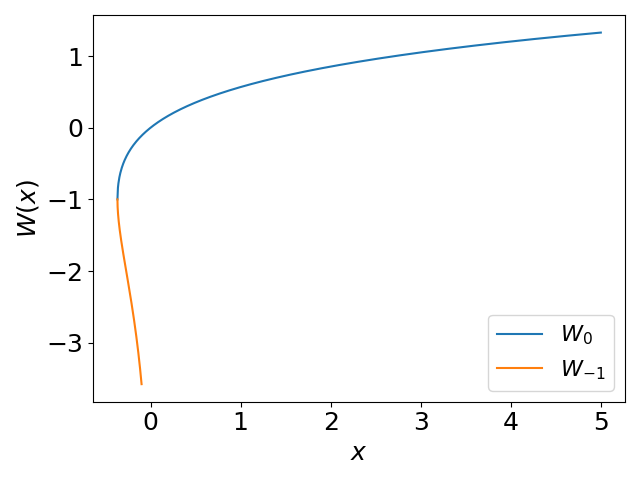
\includegraphics[width=0.6\textwidth]{figures/lambert-w.png}
	\caption{The graph of $y=W(x)$ for real $x<6$ and $y>-4$. The upper branch (blue) with $y\geq-1$ is the graph of the function $W_0(x)$ (principal branch), the lower branch (magenta) with $y\leq -1$ is the graph of the function $W_{-1}(x)$. The left most point of the curve is at $(-1/e,-1)$.}
	\label{fig:lambert-w}
\end{figure}

\subsection{Velocity Profiles}
In this research, we are interested in the stability of such plasma flow in the nozzle at equilibrium. Let's denote $n_0$ and $v_0$ as equilibrium density and equilibrium velocity, respectively. Since they are stationary (time independent) solutions to the governing equations Eq.~(\ref{eq:conservation-of-density}), (\ref{eq:conservation-of-momentum}), they satisfy the so-called equilibrium condition (nondimensionalized),
\begin{align}
	 & \pdv{z}(\frac{n_0v_0}{B}) = 0 \label{eq:equilibrium-conservation-of-density}                 \\
	 & v_0\pdv{v_0}{z} = -\frac{1}{n_0}\pdv{n_0}{z} \label{eq:equilibrium-conservation-of-momentum}
\end{align}

In this section we will solve the equilibrium velocity profile, $v_0$, from the nondimensionalized equilibrium condition, Eq.~(\ref{eq:equilibrium-conservation-of-density}) and Eq.~(\ref{eq:equilibrium-conservation-of-momentum}).
We start by substituting $\frac{1}{n_0}\pdv*{n_0}{z}$ into Eq.~(\ref{eq:equilibrium-conservation-of-density}), then it becomes
\begin{equation}
	(v_0^2-1)\pdv{v_0}{z} = -\frac{v_0}{B}\pdv{B}{z}
\end{equation}

Notice that there is a singularity at $v_0=1$, the sonic speed. Later we will devote an entire Chap.~\ref{chap:singular-perturbation} to discuss the treatment for solving eigenvalues involving this singularity.

We can solve the equation by separating the variables, i.e. $v_0$ on one side and $B$ on the other side of the equal sign. Then integrate equation with respect to $z$ and use the conditions at midpoint $B(0)=B_m, v_0(0)=v_m$ we get
\begin{equation}
	v_0^2e^{-v_0^2} = \frac{B^2}{B_m^2}v_m^2e^{-v_m^2}
\end{equation}
We can now express $v_0$ using the Lambert W function,
\begin{equation}
	v_0(z) = \left[ -W_k\left(-\frac{B(z)^2}{B_m^2}v_m^2e^{-v_m^2}\right) \right]^{1/2}
	\label{eq:velocity-profile}
\end{equation}
where the subscript $k$ of $W$ stands for branch of Lambert W function.

When considering the velocity profile of a nozzle flow, various scenarios can be distinguished based on the Mach number parameter ($v_m$) and the branch ($k$) used in the expression for the Mach number distribution, denoted as $v_0(z)$. These parameters play a crucial role in determining the flow characteristics. The selection of appropriate $v_m$ and $k$ values facilitates the control of the flow characteristics in the nozzle, allowing for the realization of various flow regimes, such as subsonic, supersonic, transonic, accelerating, or decelerating profiles. Different velocity profiles are shown in Fig.~\ref{fig:velocity-profiles}.
\begin{itemize}
	\item Subsonic profile: when $v_m < 1$ and $k = 0$, the resulting velocity profile is classified as subsonic. This means that both at the entrance and exit of the nozzle, the velocity remains subsonic, and the midpoint velocity is also less than unity ($v_m < 1$). A subsonic flow is characterized by fluid velocities that are slower than the local speed of sound. The blue and orange curves on Fig.~\ref{fig:velocity-profiles} are both subsonic profiles. As $z$ goes from $-1$ to $0$, the point $(z,W)$ moves towards the point $(-1/e, 1)$ along the $k=-1$ branch. As $z$ goes from $0$ to $1$, the point $(z, W)$ moves away $(-1/e,1)$ along the same $k=-1$ branch.
	\item Supersonic profile: when $v_m > 1$ and $k = -1$, the velocity profile corresponds to a supersonic flow. In this situation, the fluid velocities at both the entrance and exit of the nozzle are supersonic, and the midpoint velocity ($v_m$) exceeds the value of unity ($v_m > 1$). Supersonic flow is characterized by velocities that surpass the speed of sound. The purple and brown curves on Fig.~\ref{fig:velocity-profiles} are both supersonic profiles. As $z$ goes from $-1$ to $0$, the point $(z,W)$ moves towards the point $(-1/e, 1)$ along the $k=0$ branch. As $z$ goes from $0$ to $1$, the point $(z, W)$ moves away $(-1/e,1)$ along the same $k=0$ branch.
	\item Accelerating profile: when $v_m = 1$, the velocity profile becomes transonic. In this case, the midpoint velocity is exactly at the sonic threshold ($v_m = 1$), where the fluid velocity equals the local speed of sound. To achieve an accelerating velocity profile, a configuration with $k = 0$ for $z < 0$ and $k = -1$ for $z > 0$ is employed. Here, $z$ represents the spatial coordinate along the nozzle length. With this setup, the flow starts subsonically and gradually accelerates to a supersonic speed as it propagates along the nozzle. The green curve on Fig.~\ref{fig:velocity-profiles} is the accelerating profile. As $z$ goes from $-1$ to $0$, the point $(z,W)$ moves towards the point $(-1/e, 1)$ along the $k=-1$ branch. As $z$ goes from $0$ to $1$, the point $(z, W)$ moves away $(-1/e,1)$ along another branch, $k=0$.
	\item Decelerating profile: set $v_m = 1$ again, then a decelerating velocity profile can be obtained by adopting a similar approach but with reversed values of $k$. Specifically, the configuration will have $k = -1$ for $z < 0$ and $k = 0$ for $z > 0$, causing the flow to start supersonically and decelerate to subsonic velocities further down the nozzle. The red curve on Fig.~\ref{fig:velocity-profiles} is the decelerating profile. As $z$ goes from $-1$ to $0$, the point $(z,W)$ moves towards the point $(-1/e, 1)$ along the $k=0$ branch. As $z$ goes from $0$ to $1$, the point $(z, W)$ moves away $(-1/e,1)$ along another branch, $k=-1$.
\end{itemize}


\begin{figure}[htbp]
	\centering
	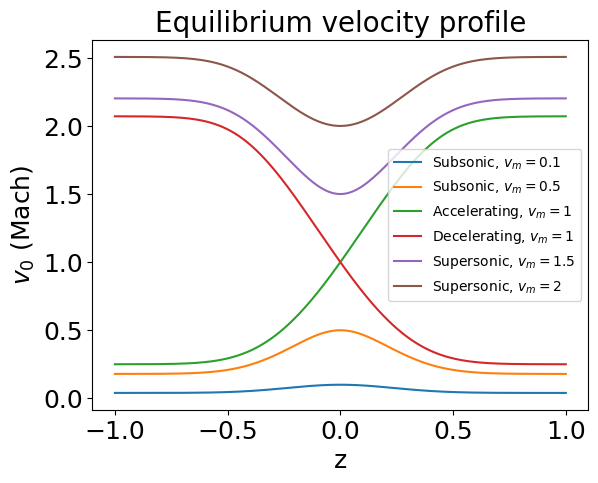
\includegraphics[width=0.7\linewidth]{figures/velocity-profiles}
	\caption{The velocity profile in the magnetic nozzle is completely determined by the midpoint mach number $v_m$ and the branch $k$. A subsonic profile can be obtained by selecting $v_m<1$ and $k=0$. On the other hand, a supersonic profile can be obtained by setting $v_m>1$ and $k=-1$. Lastly, for the transonic velocity profiles, the midpoint velocity is set to unity, $v_m=1$, and then by choose $k=0$ for $x<0$ and $k=-1$ for $x>0$ we get accelerating profile. Decelerating profile can be obtained similarly.}
	\label{fig:velocity-profiles}
\end{figure}

\section{Linearized Governing Equations}
As illustrated in Sec.\ref{sec:instability-of-plasma-flow}, it is essential to linearize the governing equations in order to investigate the linear instability of plasma. Now we are going to derive the linearized governing equations with the equilibrium conditions given in above.

Let $n = n_0(z) + \tilde{n}(z,t)$ and $v = v_0(z) + \tilde{v}(z,t)$, where $\tilde{n}$ and $\tilde{v}$ are small perturbed quantities.

We first linearize Eq.~(\ref{eq:conservation-of-density}) by setting $n=n_0+\tilde{n}$ and $v=v_0+\tilde{v}$,
\[    \pdv{(n_0+\tilde{n})}{t}
	+ (n_0+\tilde{n})\pdv{(v_0+\tilde{v})}{z}
	+ (v_0+\tilde{v})\pdv{(n_0+\tilde{n})}{z}
	- (n_0+\tilde{n})(v_0+\tilde{v})\frac{\partial_z B}{B} = 0
\]
By ignoring the nonlinear terms, we obtain
\[ \frac{1}{n_0}\pdv{\tilde{n}}{t}
	+ \pdv{v_0}{z} + \frac{\tilde{n}}{n_0}\pdv{v_0}{z} + \pdv{\tilde{v}}{z}
	+ \frac{v_0}{n_0}\pdv{n_0}{z} + \frac{\tilde{v}}{n_0}\pdv{n_0}{z} + \frac{v_0}{n_0}\pdv{\tilde{n}}{z}
	- v_0\frac{\partial_z B}{B} - \tilde{v}\frac{\partial_z B}{B} - \tilde{n}\frac{v_0}{n_0}\frac{\partial_z B}{B} = 0
\]


Using the equilibrium condition Eq.~(\ref{eq:equilibrium-conservation-of-density}), some of the terms are canceled. Moreover, the last term can be written as
\[ \tilde{n}\frac{v_0}{n_0}\frac{\partial_z B}{B} = \frac{\tilde{n}}{n_0}\left( \frac{\partial_z n_0}{n_0}v_0 + \pdv{v_0}{z} \right) \]
Now, we get the linearized conservation of mass,
\begin{equation} \label{eq:linearized-conservation-of-density}
	\frac{1}{n_0}\pdv{\tilde{n}}{t}
	+ \pdv{\tilde{v}}{z} + v_0\tilde{Y} + \tilde{v}\frac{\partial_z n_0}{n_0} - \tilde{v}\frac{\partial_z B}{B} = 0
\end{equation}
where
\[ \tilde{Y} \equiv \frac{1}{n_0}\pdv{\tilde{n}}{z} - \frac{\partial_z n_0}{n_0^2}\tilde{n} = \pdv{z}(\frac{\tilde{n}}{n_0}) \]

To linearize the conservation of momentum, we follow the same logic by substituting $n=n_0+\tilde{n}$, and $v=v_0+\tilde{v}$ in Eq.~(\ref{eq:conservation-of-momentum}),
\[ (n_0+\tilde{n})\pdv{(v_0+\tilde{v})}{t} + (n_0+\tilde{n})(v_0+\tilde{v})\pdv{(v_0+\tilde{v})}{z} = -\pdv{n}{z} \]

Again, ignore second order perturbations and rearange terms, we have
\[ \pdv{v_0}{t} + v_0\pdv{v_0}{z} + \tilde{v}\pdv{v_0}{z}
	= -\frac{1}{n_0}\pdv{n_0}{z} -\frac{1}{n_0}\pdv{\tilde{n}}{z} -v_0\frac{v_0}{z} - \frac{\tilde{n}}{n_0}v_0\pdv{v_0}{z} \]
Using the equilibrium condition Eq.~(\ref{eq:equilibrium-conservation-of-momentum}) on the RHS, we get the linearized conservation of momentum,
\begin{equation} \label{eq:linearized-conservation-of-momentum}
	\pdv{\tilde{v}}{t} + \pdv{(v_0\tilde{v})}{z} = -\tilde{Y}
\end{equation}

\section{Polynomial Eigenvalue Problem}
We can further simplify the problem by combining Eq.~(\ref{eq:linearized-conservation-of-density}) and Eq.~(\ref{eq:linearized-conservation-of-momentum}) into a single equation. We can substitute Eq.~(\ref{eq:linearized-conservation-of-momentum}) into Eq.~(\ref{eq:linearized-conservation-of-density}) to eliminate $\tilde{Y}$,

\begin{equation} \label{eq:single-governing-equation}
	\pdv{t}\frac{\tilde{n}}{n_0}
	+ \pdv{\tilde{v}}{z} - v_0\left(\pdv{t}\tilde{v}
	+ \pdv{(v_0\tilde{v})}{z}\right)
	+ \tilde{v}\frac{\partial_z n_0}{n_0}
	- \tilde{v}\frac{\partial_z B}{B}
	= 0
\end{equation}

In order to investigate the linear instability of the flow, we need to formulate it as an eigenvalue problem. To do that, we assume the perturbed density and velocity are oscillatory, i.e. $\tilde{n}, \tilde{v} \sim \exp(-i\omega t)$, where $\omega$ is the oscillation frequency of the perturbed quantities. This frequency can be a complex number.

As illustrated in Sec.\ref{sec:instability-of-plasma-flow}, the flow can be stable or unstable depending on the imaginary part of the frequency. If $\Im(\omega) > 0$, then the perturbed quantities $\tilde{n} \sim \exp(\Im(\omega) t)$, which means it grows exponentially with time, hence unstable. If $\Im(\omega) \leq 0$, then the amplitude of the perturbed quantities are either unchanged or exponentially decreasing, hence the flow is stable.

By assuming oscillatory perturbed quantities, Eq.~(\ref{eq:single-governing-equation}) becomes,
\begin{equation}
	-i\omega\frac{\tilde{n}}{n_0}
	+ \pdv{\tilde{v}}{z} - v_0\left(-i\omega\tilde{v}
	+ \pdv{(v_0\tilde{v})}{z}\right)
	+ \tilde{v}\frac{\partial_z n_0}{n_0}
	- \tilde{v}\frac{\partial_z B}{B}
	= 0
\end{equation}

Using the equilibrium condition Eq.~(\ref{eq:equilibrium-conservation-of-density}), we can eliminate the term $\partial_z B/B$,
\[
	-i\omega\frac{\tilde{n}}{n_0}
	+ \pdv{\tilde{v}}{z}
	+ v_0\left(i\omega \tilde{v} - v_0\pdv{\tilde{v}}{z} - \tilde{v}\pdv{v_0}{z} \right)
	- \tilde{v}\frac{\partial_z v_0}{v_0}
	= 0
\]

Rearrange terms, we have
\[
	-i\omega\frac{\tilde{n}}{n_0}
	+ i\omega v_0\tilde{v}
	+ (1-v_0^2)\pdv{\tilde{v}}{z}
	- \left(v_0+\frac{1}{v_0}\right)\pdv{v_0}{z}\tilde{v} = 0
\]

Now we take $\pdv*{t}$ on Eq.~(\ref{eq:linearized-conservation-of-momentum}). Recall the fact that $\tilde{Y} = \partial_z(\tilde{n}/n_0)$, we have
\[
	\omega^2\tilde{v} + i\omega\left(v_0\pdv{\tilde{v}}{z} + \tilde{v}\pdv{v_0}{z}\right)
	= \pdv{t}\pdv{z}(\frac{\tilde{n}}{n_0})
\]
Apply $\partial_t$ operator first, we get
\[
	\omega^2\tilde{v} + i\omega\left(v_0\pdv{\tilde{v}}{z} + \tilde{v}\pdv{v_0}{fz}\right)
	= \pdv{z}(-i\omega v_0\tilde{v}
	- (1-v_0^2)\pdv{\tilde{v}}{z}
	+ \left(v_0+\frac{1}{v_0}\right)\pdv{v_0}{z}\tilde{v})
\]
Expand the RHS and collect terms, we get
\begin{equation} \label{eq:polynomial-eigenvalue-problem}
	\begin{aligned}
		 & \omega^2 \tilde{v}                                          \\
		 & +2i\omega\left(v_0\pdv{}{z} + \pdv{v_0}{z}\right) \tilde{v} \\
		 & +\left[ (1-v_0^2)\pdv[2]{}{z}
			-\left(3v_0 + \frac{1}{v_0}\right)\pdv{v_0}{z}\pdv{}{z}
			- \left(1-\frac{1}{v_0^2}\right)\left(\pdv{v_0}{z}\right)^2
			- \left(v_0+\frac{1}{v_0}\right)\pdv[2]{v_0}{z} \right]\tilde{v}
		= 0
	\end{aligned}
\end{equation}

In mathematical terms, Eq.~(\ref{eq:polynomial-eigenvalue-problem}) is a polynomial eigenvalue problem, where $\omega$ is an eigenvalue to the problem, and the velocity perturbation $\tilde{v}$ is an eigenfunction associated with the eigenvalue $\omega$. In the later chapters we will discuss the methods to tackle this problem.

\section{Analytical Solutions to Constant Velocity Case}
In this section we are going to tackle the simplest case of the polynomial eigenvalue problem, Eq.~(\ref{eq:polynomial-eigenvalue-problem}), the constant velocity case.

The constant velocity profile can be viewed as the limit of $v_0(z)$ as the spread of magnetic field goes to infinity, $\delta\to\infty$. As the parameter $\delta$ approaches infinity, the width of the magnetic field enlarges and eventually becomes flat. In other words, a constant magnetic field. We can easily see that the velocity profile $v_0(z)$ becomes a constant as well.

If we set the velocity profile of the equilibrium flow to constant $v_0=\text{const}$, then Eq.~(\ref{eq:polynomial-eigenvalue-problem}) becomes a simple boundary value problem with second order constant coefficients differential equation.

\begin{equation} \label{eq:constant-v-problem-dirichlet}
	\omega^2\tilde{v} + 2i\omega v_0\pdv{\tilde{v}}{z} + (1-v_0^2)\pdv[2]{\tilde{v}}{z} = 0
\end{equation}

We need two boundary values in order to uniquely determine the solution (up to a constant). In the following subsections, we will solve Eq.~(\ref{eq:polynomial-eigenvalue-problem}) with constant velocity under two sets of boundary conditions, Dirichlet and fixed-open boundary condition.

\subsection{Dirichlet Boundary}
In this subsection, the so-called Dirichlet boundary condition will be used. It has the name because the function values are fixed at the two ends of the nozzle,
\[ \tilde{v}(-1) = \tilde{v}(1) = 0 \]
At the left end (entrance of the nozzle), $z=-1$, we assume there are no perturbations. As for the right end (exit of the nozzle), $z=1$, setting the velocity perturbation to 0 might not be the best boundary condition to describe the physical process of the plasma flow in the nozzle, it nevertheless serves as a starting point to the problem and is also useful to test numerical solutions.

With the two boundary conditions, we find the solution to this problem,
\begin{equation} \label{eq:constant-v-solution-dirichlet}
	\tilde{v}(z) = C\left[ \exp\left(i\omega\frac{z+1}{v_0+1}\right) - \exp\left(i\omega\frac{z+1}{v_0-1}\right) \right]
\end{equation}
where $C\in\mathbb{C}$ is a complex constant, and the frequencies (eigenvalues) are
\begin{equation}
	\omega_n = n\pi(1-v_0^2)/2,\quad n\in\mathbb{Z}
	\label{eq:eigvals-constant-v-dirichlet}
\end{equation}
The results are plotted in Fig.~\ref{fig:exact-v-dirichlet} This result tells us that the flow in a magnetic nozzle with uniform magnetic field is stable regardless the velocity $v_0$ for constant velocity case.

This solution is exact, we will use this to benchmark the simulation results in later chapter.

\begin{figure}[htbp]
	\centering
	\begin{subfigure}{0.5\textwidth}
		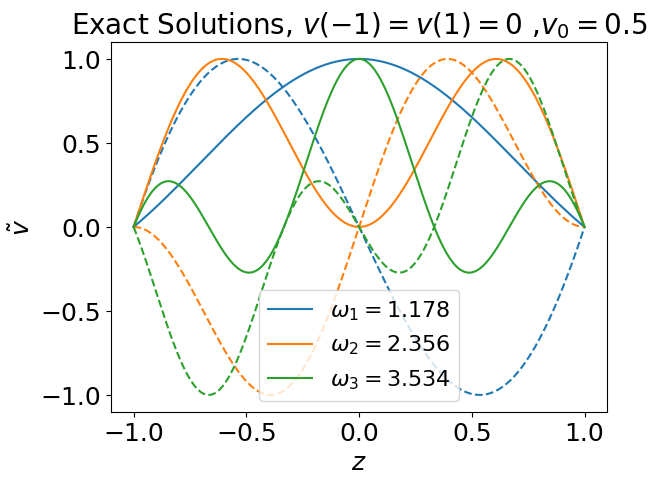
\includegraphics[width=\linewidth]{figures/exact-fixed-fixed-v0=0.5}
		\caption{Subsonic}
	\end{subfigure}%
	\begin{subfigure}{0.5\textwidth}
		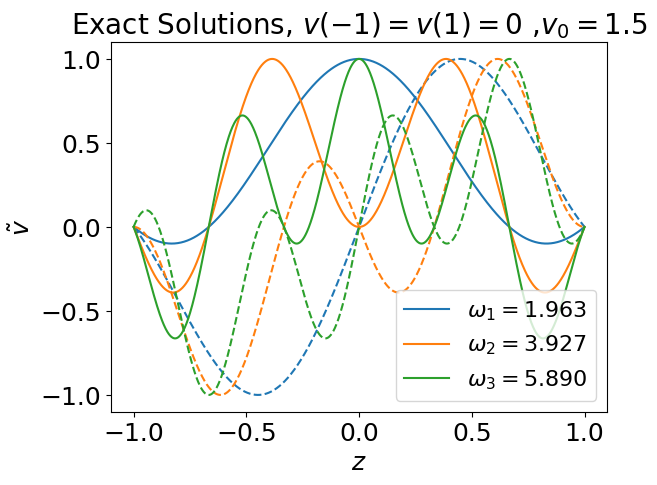
\includegraphics[width=\linewidth]{figures/exact-fixed-fixed-v0=1.5}
		\caption{Supersonic}
	\end{subfigure}
	\caption{The plots show the first three non-zero exact solutions to Eq.~(\ref{eq:constant-v-problem-dirichlet}) for both subsonic and supersonic case. These solutions are stable.}
	\label{fig:exact-v-dirichlet}
\end{figure}

\subsection{Fixed-Open Boundary}
Fixed-Open boundary condition assumes that there are no perturbations at the entrance of the nozzle, and it is free on the exit of the nozzle.

\begin{equation} \label{eq:constant-v-problem-fixed-open}
	\omega^2\tilde{v} + 2i\omega v_0\pdv{\tilde{v}}{z} + (1-v_0^2)\pdv[2]{\tilde{v}}{z} = 0
	\quad
	\tilde{v}(-1) = \pdv{\tilde{v}}{z}\,(1) = 0
\end{equation}

The form of the solution to this problem is the same as Eq.~(\ref{eq:constant-v-solution-dirichlet}), the only difference is the eigenvalues. In this case, the eigenvalues are
\begin{equation}
	\omega_n = (v_0^2 - 1) \left[\frac{n\pi}{2} - \frac{1}{4}i\ln(\frac{v_0-1}{v_0+1})\right], \quad n\in\mathbb{Z}
	\label{eq:eigvals-constant-v-fixed-open}
\end{equation}
The growth rate is independent of the mode number $n$, and it is always $\ln((v_0-1)/(v_0+1))$. It is is positive for any $v_0\neq 1$. Therefore,
\begin{itemize}
	\item If $v_0<1$, then $\Im(\omega)<0$, it's damped oscillation, hence stable.
	\item If $v_0>1$, then $\Im(\omega)>0$, it's unstable.
\end{itemize}

\begin{figure}[htbp]
	\centering
	\begin{subfigure}{0.5\textwidth}
		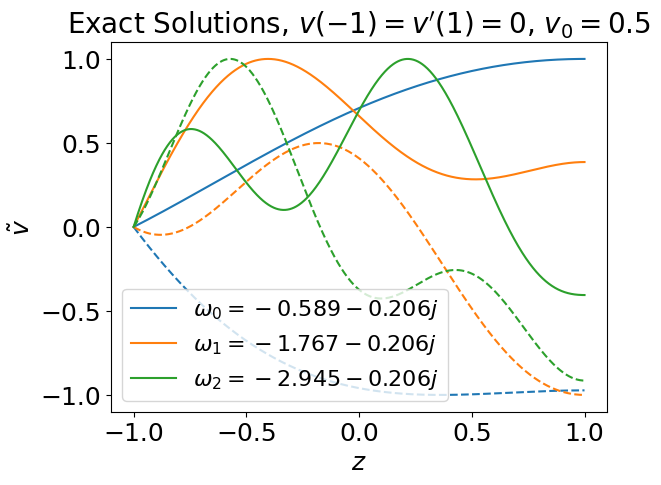
\includegraphics[width=\linewidth]{figures/exact-fixed-open-v0=0.5}
		\caption{Subsonic, stable flow.}
	\end{subfigure}%
	\begin{subfigure}{0.5\textwidth}
		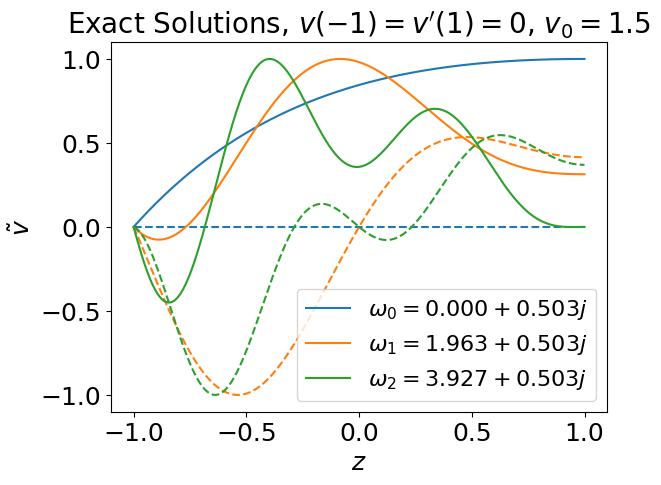
\includegraphics[width=\linewidth]{figures/exact-fixed-open-v0=1.5}
		\caption{Supersonic, unstable flow.}
	\end{subfigure}
	\caption{The plots show the first three exact solutions to Eq.~(\ref{eq:constant-v-problem-fixed-open}) for both subsonic and supersonic case. The flow is stable for subsonic case and unstable for supersonic case.}
	\label{fig:exact-v-fixed-open}
\end{figure}

\chapter{Spectral Method} \label{chap:spectral-method}
In Chap.~\ref{chap:polynomial-eigenvalue-problem}, we explored the analytical solutions, including eigenvalues and eigenfunctions, to Eq.~(\ref{eq:constant-v-problem}), a special case of a more general polynomial eigenvalue problem Eq.~(\ref{eq:polynomial-eigenvalue-problem}). As we can see, it is nearly impossible to solve Eq.~(\ref{eq:polynomial-eigenvalue-problem}) analytically. Hence, we need numerical methods to investigate the instability of plasma flow with spatial varying velocity profile. Spectral methods is a suitable tool for our problem.

Spectral method is an important tool for solving problems related to partial differential equations. It can provide superior accuracy compare to other local methods such as finite difference \cite{shen_tang_etal_spectral_2011}. In this thesis, we are going to solve a polynomial eigenvalue problem, i.e. Eq.~(\ref{eq:polynomial-eigenvalue-problem}) together with specific boundary conditions.

Suppose the velocity perturbation $\tilde{v}$ can be approximated by some orthogonal basis functions $\{u_k(z)\}_{k=1}^{\infty}$ on $-1\leq z\leq 1$,
\begin{equation}
	\tilde{v} = \sum_{k=0}^{N} c_ku_k(z),
\end{equation}
where $c_k$ are coefficients to be determined. There are different choices for $u_k(z)$ including but not limited to \cite{shen_tang_etal_spectral_2011},
\begin{itemize}
	\item $u_k(z)=T_k(z)$ (Chebyshev spectral method)
	\item $u_k(z)=L_k(z)$ (Legendre spectral method)
	\item $u_k(z)=H_k(z)$ (Hermite spectral method)
\end{itemize}
where $T_k$, $L_k$ and $H_k$ are Chebyshev, Legendre, and Hermite polynomials of degree $k$.

Using the above approximation in Eq.~(\ref{eq:polynomial-eigenvalue-problem}), and take the inner product with some other test functions $\{\psi_k(z)\}$ on $[-1,1]$, the left-hand side of Eq.~(\ref{eq:polynomial-eigenvalue-problem}) becomes a matrix equation,
\begin{equation}
	(\omega^2\mathbf{1} + \omega\mathbf{M} + \mathbf{N})\mathbf{c} = \mathbf{0},
	\label{eq:pep-matrix-equation}
\end{equation}
where $\mathbf{c} = [c_0, \cdots, c_N]^T$ is a vector of coefficients, and
\begin{align}
	M_{jk} & = 2i\int_{-1}^{1}dz \; \psi_{j}\left(v_0\pdv{}{z} +\pdv{v_0}{z} \right)u_{k}
	\label{eq:operator-matrix-M}                                                          \\
	N_{jk} & = \int_{-1}^{1}dz \; \psi_{j} \left[(1-v_0^2)\pdv[2]{}{z}
		-\left(3v_0 + \frac{1}{v_0}\right)\pdv{v_0}{z}\pdv{}{z}
		- \left(1-\frac{1}{v_0^2}\right)\left(\pdv{v_0}{z}\right)^2
		- \left(v_0+\frac{1}{v_0}\right)\pdv[2]{v_0}{z}\right] u_{k}
	\label{eq:operator-matrix-N}
\end{align}

Depending on the choice of the test function, spectral method can be further classified \cite{shen_tang_etal_spectral_2011},
\begin{itemize}
	\item Galerkin: The test functions are the same as the trial ones, i.e. $\psi_k=u_k$.
	\item Collocation:  The test functions $\{\psi_k\}$ are Lagrange basis polynomials such that $\psi_k(z_j)=\delta_{jk}$, where ${z_j}$ are preassigned collocation points.
\end{itemize}

To solve Eq.~(\ref{eq:pep-matrix-equation}), we simply augment the coefficient vector to $[\mathbf{c}, \omega\mathbf{c}]^T$. Then the matrix equation can be written as an algebraic eigenvalue problem,
\begin{equation} \label{eq:eigenvalue-problem}
	\mqty[ \mathbf{0} & \mathbf{1}\\ -\mathbf{N} & -\mathbf{M} ]\mqty[ \mathbf{c}\\ \omega\mathbf{c}] = \omega\mqty[ \mathbf{c}\\ \omega\mathbf{c}].
\end{equation}
We can apply standard eigenvalue problem solver to this question to obtain the eigenvalues $\omega$ and their corresponding eigenvectors $[\mathbf{c}, \omega\mathbf{c}]^T$. Therefore, the eigenfunctions $\tilde{v} = \sum_k c_ku_k(z)$ to the original problem can be recovered by extracting coefficients $\mathbf{c}$ from the eigenvectors.

\section{Spectral Collocation Method}
One of the methods we are going to use is called the Chebyshev collocation method.
Given a set of Chebyshev points, $\{z_j=\cos(j\pi/N)\}_{j=0}^{N}$, and let $\{h_j\}$ be the Lagrange basis polynomials associated with $\{z_j\}_{j=0}^{N}$, and define matrix $D_{kj} = h'_j(z_k)$. By setting $\tilde{v}(z) = \sum_{j=0}^{N}c_jh_j(z)$, we see that
\begin{align}
	\tilde{v}(z_k)   & = \sum_{j=0}^{N}\tilde{v}_jh_j(z_k) = c_k                         \\
	\tilde{v}'(z_k)  & = \sum_{j=0}^{N}\tilde{v}_jh'_j(z_k) = \sum_{j=0}^{N}D_{kj}c_j    \\
	\tilde{v}''(z_k) & = \sum_{j=0}^{N}\tilde{v}_jh''_j(z_k) = \sum_{j=0}^{N}D^2_{kj}c_j
\end{align}
We see that the coefficient vector $\mathbf{c}$ becomes a vector containing the values of $\tilde{v}$ evaluated at the collocation points, i.e. $\mathbf{c}=[v(z_0), \cdots, v(z_N)]^T$, and the matrix $D$ and $D^2$ act as the differential operators $\pdv{z}$ and $\pdv[2]{z}$, respectively. The matrix $D$ is called Chebyshev differentiation matrix since it acts as $\pdv{z}$ and evaluates at Chebyshev points.

\subsubsection*{Chebyshev Differentiation Matrix}
The Chebyshev differentiation matrix finds the derivative of the Lagrange interpolant of the given data points $(z_j,\tilde{v}(z_j))$ where $\{z_j = \cos(j\pi/N)\}_{j=0}^{N}$ are the Chebyshev points. Suppose $\mathbf{v} = [v(z_0), \cdots, v(z_N)]^T$, then the $N$-point, $D_N$, Chebyshev differentiation matrix gives $D_N\mathbf{v} \approx [v'(z_0),\cdots, v'(z_N)]^T$. Higher order differentiation can be achieved by taking powers of $D_N$. Thanks to \cite{trefethen_spectral_2000}, the construction of Chebyshev differentiation matrix is given in Fig.~\ref{fig:chebyshev-differentiation-matrix}.

If we instead use the equal-spaced points, $\{z_j=2j/N\}_{j=0}^{N}$, then the matrix defined by $D_{kj} = h'_j(x_k)$ will be the usual finite difference differentiation matrix. However, Chebyshev differentiation matrix has superior accuracy due to the wise choice of collocation points. On Fig.~\ref{fig:chebyshev-vs-fd} we see that the Chebyshev achieve higher accuracy.

\begin{figure} [htbp]
	\centering
	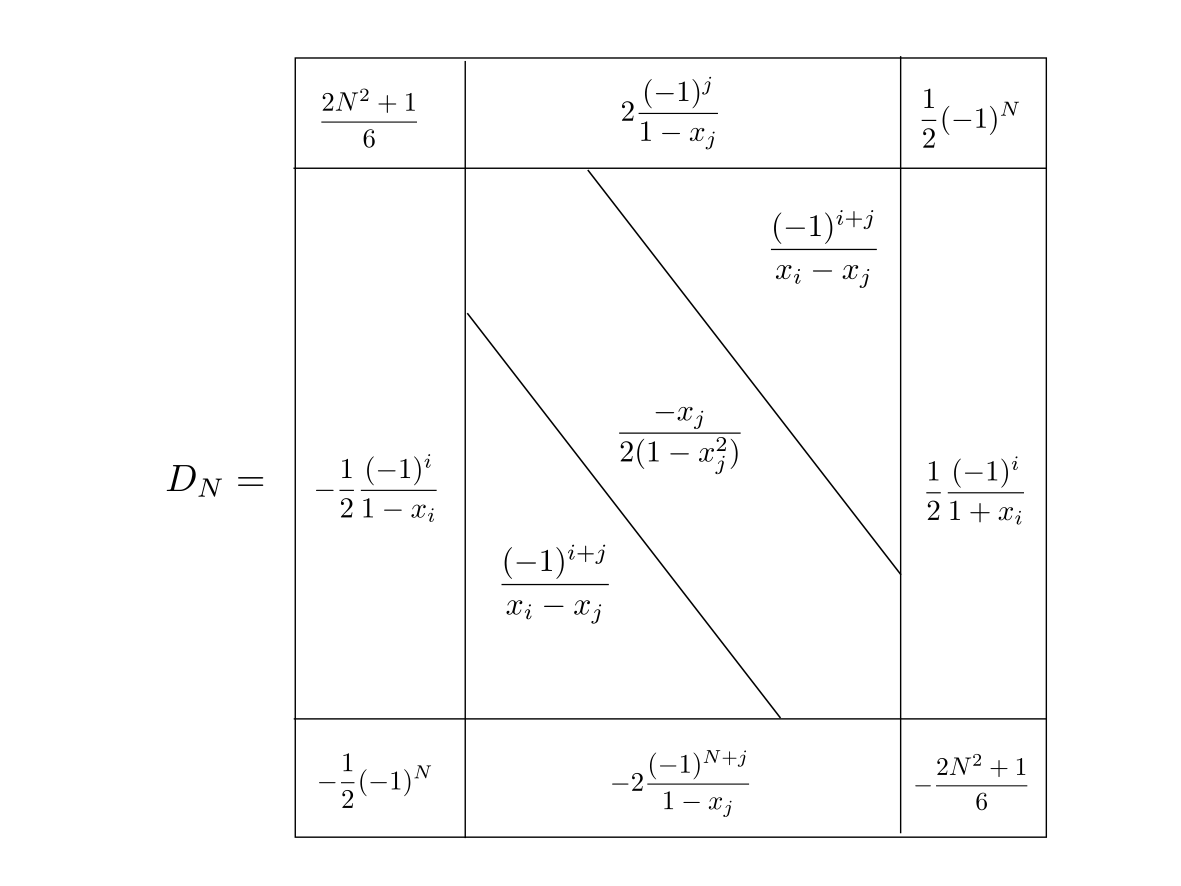
\includegraphics[width=\textwidth]{figures/chebyshev-differentiation-matrix.png}
	\caption{Construction of $N$-point Chebyshev differentiation matrix. The nodes $x_j = \cos(j\pi/N)$ are Chebyshev points. Adapted from \cite{trefethen_spectral_2000}.}
	\label{fig:chebyshev-differentiation-matrix}
\end{figure}

\begin{figure}
	\centering
	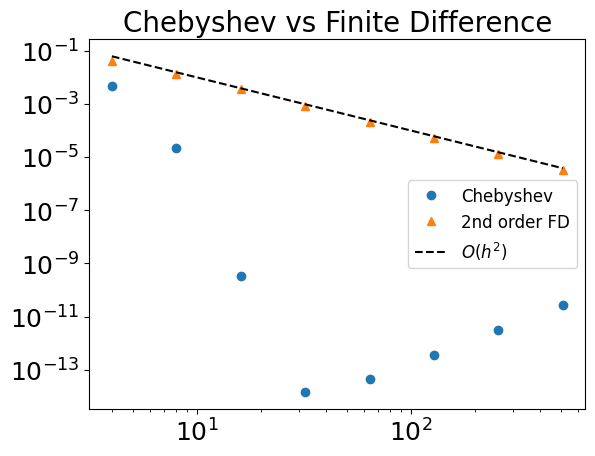
\includegraphics[width=0.7\textwidth]{figures/chebyshev-vs-fd.png}
	\caption{Comparison of accuracy between Chebyshev differentiation matrix and 2nd order finite difference differentiation matrix. Both methods are applied to compute the derivative of function $f(x)=\ln(2+\sin(x))$ on $[-1,1]$ using different resolutions, i.e. number of points $N$. We see that Chebyshev achieve higher accuracy using same amount of points.}
	\label{fig:chebyshev-vs-fd}
\end{figure}

\subsubsection*{Dirichlet Boundary}
To implement Dirichlet boundary condition, $\tilde{v}(\pm 1)=0$, to Eq.~(\ref{eq:pep-matrix-equation}), we only need to remove the first and last columns and rows of each matrix, $\mathbf{0,1,M}$, and $\mathbf{N}$. The reason is originated from the Chebyshev differentiation matrix, Fig.~\ref{fig:chebyshev-differentiation-dirichlet}. For a $(N+1)\times(N+1)$ Chebyshev differentiation matrix $D_N$, the first and last row has no effect since the first and last value of $\tilde{v}$ are $0$. We only need the interior of $D_N$ which is an $N\times N$ matrix. After solving Eq.~(\ref{eq:pep-matrix-equation}), we get the eigenvalues $\omega$ and their associated eigenfunctions evaluated at the interior collocation points $\mathbf{c} = [\tilde{v}_1,\cdots,\tilde{v}_{N-1}]^T$. We will need to prepend and append 0 to the eigenfunctions, $[0, \tilde{v}_1,\cdots\tilde{v}_{N-1}, 0]^T$. Listing.~\ref{code:spectral-collocation-dirichlet} has the pseudocode for solving Eq.~(\ref{eq:pep-matrix-equation}).

\begin{figure} [htpb]
	\centering
	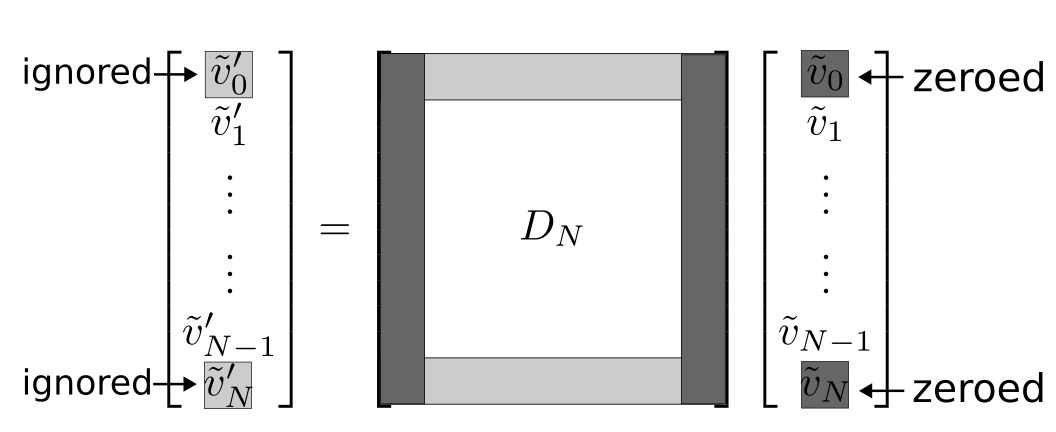
\includegraphics[width=0.7\textwidth]{figures/chebyshev-differentiation-dirichlet.png}
	\caption{Since the function $v$ is zero at $x_0$ and  $x_N$, the first and last columns has no effect and the same argument applies to first and last rows. Adapted from \cite{trefethen_spectral_2000}.}
	\label{fig:chebyshev-differentiation-dirichlet}
\end{figure}


\begin{lstlisting}[language=Python, float, floatplacement=H, caption={Pseudocode for solving polynomial eigenvalue problem using spectral collocation with Dirichlet boundary condition.}, label=code:spectral-collocation-dirichlet]
import numpy as np
# collocation points, differentiation matrices	
N = 101 # number of points
x, D1, D2 = Chebyshev(N) 
# solve polynomial eigenvalue problem
A11 = np.zeros_like(D1)
A12 = np.eye(*D1.shape)
A21 = -np.diag(1-v0**2)@D2 \
        + np.diag((3*v0 + 1/v0)*(D1@v0))@D1 \
        + np.diag((1-1/v0**2)*(D1@v0)**2) \
        + np.diag((v0+1/v0)*(D2@v0)) 
A22 = -2j*(np.diag(v0)@D1 + np.diag(D1@v0))
A = np.block([[A11[1:-1,1:-1], A12[1:-1,1:-1]],
              [A21[1:-1,1:-1], A22[1:-1,1:-1]]])
omega, V = np.linalg.eig(A)
# pad two ends of eigenfunctions by 0 (dirichlet boundary)
V = np.pad(V,((1,1),(0,0)))
\end{lstlisting}

\subsubsection*{Fixed-Open Boundary}
To implement fixed-open boundary condition, i.e. $\tilde{v}(-1)=\tilde{v}'(1)=0$. Notice that $\tilde{v}'(-1)$ can be expressed as,
\begin{equation}
	0 = \tilde{v}'(1) = \sum_{j=0}^{N}D_{ij}\tilde{v}_j,
\end{equation}
where $\tilde{v}_j=\tilde{v}(z_j)$ is the evaluation of $\tilde{v}$ at Chebyshev points $z_j=\cos(j\pi/N)$. By rearranging the terms, we get the expression of $\tilde{v}_0$ in terms of $\tilde{v}$ at other collocation points.
\begin{equation}
	\tilde{v}_0 = -\frac{1}{D_{00}}\sum_{j=1}^{N} D_{0j}\tilde{v}_j.
	\label{eq:expression-for-first-value}
\end{equation}
To incorporate this information into the differentiation matrix, we modify the expressions for evaluating the derivatives at point $x_1$,
\begin{align}
	\tilde{v}'_{1}  & = \sum_{j=0}^{N}D_{1j}\tilde{v}_j = \sum_{j=1}^{N}\left(D_{1j} - \frac{D_{10}}{D_{00}}D_{0j}\right)\tilde{v}_j        \\
	\tilde{v}''_{1} & = \sum_{j=0}^{N}D^2_{1j}\tilde{v}_j = \sum_{j=1}^{N}\left(D^2_{1j} - \frac{D^2_{10}}{D_{00}}D_{0j}\right)\tilde{v}_j.
\end{align}
This indicates the new differentiation matrices should be
\begin{align}
	D'_{ij} = \begin{cases}
		          D_{ij}, \quad                               & \text{if $i\neq 1$} \\
		          D_{1j} - \frac{D_{10}}{D_{00}}D_{0j}, \quad & \text{if $i=1$}
	          \end{cases} \\
	D'^2_{ij} = \begin{cases}
		            D^2_{ij}, \quad                                 & \text{if $i\neq 1$} \\
		            D^2_{1j} - \frac{D^2_{10}}{D_{00}}D_{0j}, \quad & \text{if $i=1$}
	            \end{cases}
\end{align}
After getting the eigenfunctions $\mathbf{c} = [\tilde{v}_1, \cdots, \tilde{v}_N]^T$, we need to prepend $\tilde{v}_0$ to $\mathbf{c}$ using Eq.~(\ref{eq:expression-for-first-value}). See Listing.~\ref{code:spectral-collocation-fixed-open} for pseudocode.


\begin{lstlisting}[language=Python, float, floatplacement=H, caption={Pseudocode for solving polynomial eigenvalue problem using spectral collocation with fixed-open boundary condition.}, label=code:spectral-collocation-fixed-open]
import numpy as np
# collocation points, differentiation matrices	
N = 101 # number of points
x, D1, D2 = Chebyshev(N)	
# modify second row to ensure v'(1)=0 
D1v = D1
D2v = D2
D1v[1,:] = D1[1,:] - D1[1,0]/D1[0,0]*D1[0,:]
D2v[1,:] = D2[1,:] - D2[1,0]/D1[0,0]*D1[0,:]
# only the differential operators acting on v needs to be modified
A11 = np.zeros_like(D1)
A12 = np.eye(*D1.shape)
A21 = -np.diag(1-v0**2)@D2v \
        + np.diag((3*v0 + 1/v0)*(D1@v0))@D1v \
        + np.diag((1-1/v0**2)*(D1@v0)**2) \
        + np.diag((v0+1/v0)*(D2@v0))
A22 = -2j*(np.diag(v0)@D1v + np.diag(D1@v0))
A = np.block([[A11[:-1,:-1], A12[:-1,:-1]],
              [A21[:-1,:-1], A22[:-1,:-1]]])
omega, V = np.linalg.eig(A)
# add v(1) to eigenfunctions
V = np.pad(V,((1,0),(0,0)))
for j in range(V.shape[1]):
    V[0,j] = -(D1[0,1:]@V[1:,j])/D1[0,0]
\end{lstlisting}


\section{Spectral Galerkin Method}
Another spectral method we used in the numerical experiments is the Legendre-Galerkin method. Meaning that the basis functions are chosen to be the compact combinations of Legendre polynomials \cite{shen_tang_etal_spectral_2011},
\begin{equation}
	u_k(z) = L_k(z) + a_kL_{k+1}(z) + b_kL_{k+2}(z),
\end{equation}
where the parameters $\{a_k,b_k\}$ are chosen to satisfy the boundary conditions. The test functions are the same as the basis functions.

Suppose the boundary conditions are
\[ a_{-}\tilde{v}(-1) + b_{-}\tilde{v}'(-1) = 0, a_{+}\tilde{v}(1) + b_{+}\tilde{v}'(1) = 0.  \]
Then the parameters $\{a_k,b_k\}$ can be worked out by simple linear algebra,
\begin{equation}
	\begin{aligned}
		a_k & = \frac{(2k+3)(a_{+}b_{-} + a_{-}b_{+})}{\text{DET}_k}                                              \\
		b_k & = \frac{-2a_{-}a_{+} + (k+1)^2(a_{+}b_{-} - a_{-}b_{+}) + b_{-}b_{+}k(k+1)^2(k+2)/2}{\text{DET}_k},
	\end{aligned}
\end{equation}
where $\text{DET}_k = 2a_{+}a_{-} + a_{-}b_{+}(k+2)^2 - a_{+}b_{-}(k+2)^2 - b_{-}b_{+}(k+1)(k+2)^2(k+3)/2$.

\subsubsection*{Dirichlet Boundary}
\begin{figure} [htbp]
	\centering
	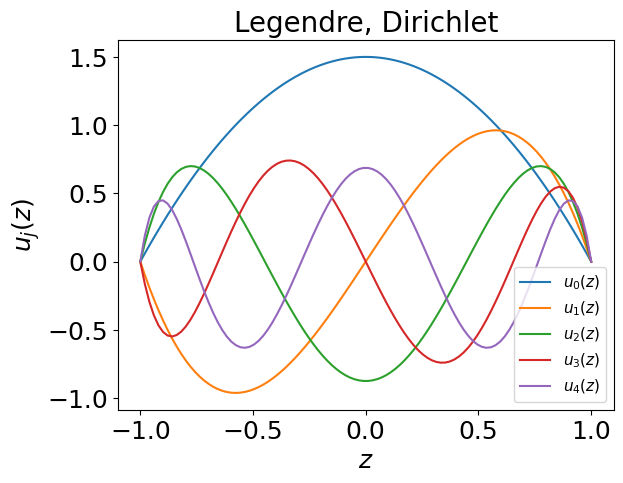
\includegraphics[width=0.7\textwidth]{figures/legendre-dirichlet.png}
	\caption{Compact Legendre combinations satisfying Dirichlet boundary condition.}
	\label{fig:legendre-dirichlet}
\end{figure}
The necessary parameters to make $u_k(\pm 1) = 0$ are $a_k=0, b_k=-1$. The basis functions are therefore,
\begin{equation}
	u_k(z) = L_k(z) - L_{k+2}(z).
\end{equation}
The first 5 basis functions are shown in Fig.~\ref{fig:legendre-dirichlet}.

\subsubsection*{Fixed-Open Boundary}
\begin{figure} [htbp]
	\centering
	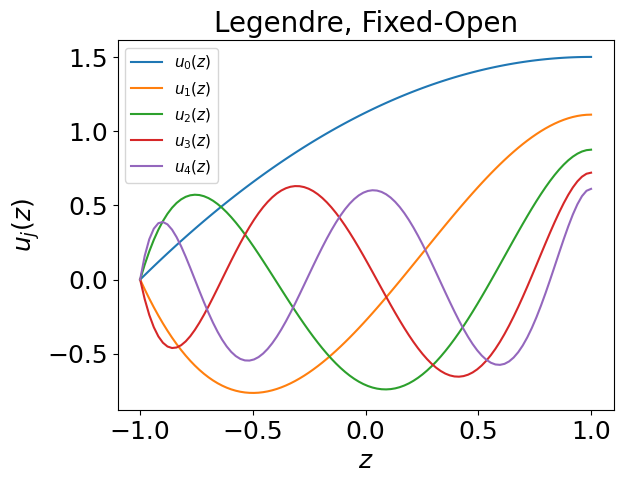
\includegraphics[width=0.7\textwidth]{figures/legendre-fixed-open.png}
	\caption{Compact Legendre combinations satisfying fixed-open boundary condition.}
	\label{fig:legendre-fixed-open}
\end{figure}
The necessary parameters to make $u_k(-1)=u_k'(1)=0$ are $a_k=(2k+3)/(k+2)^2, b_k=-(k+1)^2/(k+2)^2$. The basis functions are therefore,
\begin{equation}
	u_k(z) = L_k(z) + \frac{2k+3}{(k+2)^2}L_{k+1}(z) - \frac{(k+1)^2}{(k+2)^2}L_{k+2}(z)
\end{equation}
The first 5 basis functions are shown in Fig.~\ref{fig:legendre-fixed-open}.

By setting $\tilde{v}(z) = \sum_{j=0}^{N} c_ku_k(z)$, $\tilde{v}$ satisfies the boundary conditions automatically. There is no need to modify the matrices in Eq.~(\ref{eq:pep-matrix-equation}).

To evaluate the matrix elements, inner products are calculated by numerical integration, in this thesis Simpson's rule is used. Eq.~(\ref{eq:operator-matrix-M}) and Eq.~(\ref{eq:operator-matrix-N}) become

\begin{align}
	M_{jk} & = 2i \sum_{m}^{M} w_m \Delta z_m \left[\psi_{j}\left(v_0\pdv{}{z} +\pdv{v_0}{z} \right)u_{k}\right]_{z_m} \\
	N_{jk} & = \sum_{m}^{M} w_m \Delta z_m \left\{
	\psi_{j} \left[(1-v_0^2)\pdv[2]{}{z} -\left(3v_0 + \frac{1}{v_0}\right)\pdv{v_0}{z}\pdv{}{z}
		- \left(1-\frac{1}{v_0^2}\right)\left(\pdv{v_0}{z}\right)^2 - \left(v_0+\frac{1}{v_0}\right)\pdv[2]{v_0}{z}\right] u_{k} \right\}_{z_m},
\end{align}
where $M$ is the number of points, $\Delta z_m = 2/M$, and $w_m$ are coefficients corresponding to the quadrature rule employed. In this case,
\begin{equation}
	w_n = \begin{cases}
		1/3, \text{if $m=0,M$}    \\
		4/3, \text{if $m$ is odd} \\
		2/3, \text{if $m\neq 0,M$ and $m$ is even}.
	\end{cases}
\end{equation}

After solving Eq.~(\ref{eq:pep-matrix-equation}), the eigenvector $\mathbf{c}$ can be used to reconstruct the eigenfunctions. See Listing.~\ref{code:spectral-galerkin} for more details.

\begin{lstlisting}[language=Python, float, floatplacement=H, caption={Pseudocode for solving polynomial eigenvalue problem using Lengendre-Galerkin method}, label=code:spectral-galerkin]
import numpy as np
from scipy.special import lengendre # lengendre polynomials
from scipy.integrate import simpson # simpson quadrature
# collocation points, differentiation matrices
N = 25 # number of basis functions
M = 101 # number of points
x, D1, D2 = Chebyshev(M, "symmetric", "CH")
# use this basis for drichlet boundary
u = lambda x,k: (legendre(k) + (2*k+3)/(k+2)**2*legendre(k+1) - (k+1)**2/(k+2)**2*legendre(k+2))(x)
# use this basis for fixed-open boundary
u = lambda x,k: (legendre(k) - legendre(k+2))(x)
# solve polynomial eigenvalue problem
A11 = np.zeros_like(D1)
A12 = np.eye(*D1.shape)
A21 = np.zeros((N,N),dtype=complex)
A22 = np.zeros((N,N),dtype=complex)
for i in range(N):
    for j in range(N):
		A21[i,j] = simpson(
			- u(x,i)*(1-v0**2)*(D2@u(x,j))
			+ u(x,i)*(3*v0+1/v0)*(D1@v0)*(D1@u(x,j))
			+ u(x,i)*(1-1/v0**2)*(D1@v0)**2*u(x,j) 
			+ u(x,i)*(v0+1/v0)*(D2@v0)*u(x,j),
			x=x)
		A22[i,j] = -2j*simpson(u(x,i)*v0*(D1@u(x,j)) + u(x,i)*(D1@v0)*u(x,j),x=x)
A = np.block([[A11, A12],
              [A21, A22]])
omega, C = np.linalg.eig(A)
# construct eigenfunctions
V = np.zeros((x.size, C.shape[1]),dtype=complex)
for i in range(C.shape[1]):
    for k in range(N):
        V[:, i] += C[k,i]*u(x, k)
\end{lstlisting}


\section{Spectral Theory in Finite-Dimensional Normed Spaces}
Spectral method transforms the polynomial eigenvalue problem to an algebraic eigenvalue problem. For completion, some important linear algebra results are included in this section.

Let $X$ be a finite dimensional normed space and $\hat{T}: X \to X$ a linear operator. Since any linear operator can be represented by a matrix, the spectral theory of $\hat{T}$ is essentially matrix eigenvalue theory \cite{kreyszig_introductory_1978}. Let $A$ be a matrix representation of $\hat{T}$, then we have the definition.

\begin{definition} [Kryszig \cite{kreyszig_introductory_1978}]
	An eigenvalue of a square matrix $A$ is a complex number $\lambda$ such that
	\[ Ax = \lambda x \]
	has a solution $x\neq 0$.This $x$ is called an \textbf{eigenvector} of $A$ corresponding to that eigenvalue $\lambda$.The set $\sigma(A)$ of all eigenvalues of $A$ is called the \textbf{spectrum} of $A$. Its complement $\rho(A) = \mathbb{C}-\sigma(A)$ in the complex plane is called the \textbf{resolvent} set of $A$.
\end{definition}

By choosing different bases in $X$, we can have different matrix representation of $\hat{T}$. We need to make sure the eigenvalues of a linear operator is independent of the basis chosen. Fortunately, a theorem ensures that.

\begin{theorem} [Kryszig \cite{kreyszig_introductory_1978}]
	All matrices representing a given linear operator $\hat{T}: X \to X$ on a finite dimensional normed space $X$ relative to various bases for $X$ have the same eigenvalues.
\end{theorem}


Moreover, we don't need to worry about the existence of eigenvalues of a linear operator. The following theorem shows the existence of them.
\begin{theorem} [Kryszig \cite{kreyszig_introductory_1978}]
	A linear operator on a finite dimensional complex normed space $X\neq{O}$ has at least one eigenvalue.
\end{theorem}

\section{Spectral Pollution and Spurious Modes}
In this section, we will discuss an important phenomenon we observe throughout the numerical experiments using spectral method. It is the phenomenon of spectral pollution. Then we will provide a method to filter these spurious modes.

Spectral pollution refers to the phenomenon which some eigenvalues are not converging to the correct value when the mesh density is increased. The wrong eigenvalues are referred as spurious modes. When solving eigenvalue problems using spectral methods with finite difference or finite element approximations, spectral pollution might occur \cite{llobet_spectral_1990}. The cause of the spectral pollution is originated from the improper discretization of the differential operators. In the following sections, we are going to take a closer look at the differential operators in finite difference method, and reveal the occurrence of spurious modes when solving Eq.~(\ref{eq:constant-v-problem}) with supersonic velocity profile.

\subsection{Analysis of Numerical Spectrum} \label{sec:analysis-of-numerical-spectrum}
In this section, we will analyze the analytical and numerical dispersion relation of the following problem,
\[
	\omega^2\tilde{v} + 2i\omega v_0\pdv{\tilde{v}}{z} + (1-v_0^2)\pdv[2]{\tilde{v}}{z} = 0, \quad v(\pm 1) = 0
\]

It is a special case, i.e. $v_0=$constant, of a more general problem Eq.~(\ref{eq:polynomial-eigenvalue-problem}). The analytical dispersion relation can be obtained by substituting $\tilde{v} = \exp(-i\omega t + kx)$ into the above equation,
\begin{equation} \label{dispersion-relation}
	\omega = k(v_0 \pm 1).
\end{equation}
The dispersion relation suggests that the eigenvalue $\omega$ should be real.

Now let's analyze the dispersion relation produced by finite difference. To do this we need to first understand the effect of the differential operators on function $\tilde{v}$ in finite difference. If we assume $\tilde{v}\sim \exp(ikx)$, and let $\beta\equiv kh/2$. Then in finite difference discretization scheme, the differential operators $\dv*[n]{z}$ are equivalent to the following factors \cite{llobet_spectral_1990},
\begin{equation}
	\begin{aligned}
		\dv[0]{z} \quad \to \quad & G_0 = 1                                                               \\
		\dv[1]{z} \quad \to \quad & G_1 = [\exp(2i\beta)-\exp(-2i\beta)]/2h = (i/h)\sin(2\beta)           \\
		\dv[2]{z} \quad \to \quad & G_2 = [\exp(2i\beta)-2-\exp(-2i\beta)]/h^2 = (2/h^2)(\cos(2\beta)-1).
	\end{aligned}
	\label{eq:G-operator}
\end{equation}

Using the G-operators, Eq.~(\ref{eq:G-operator}), the discretized equation of Eq.~(\ref{eq:constant-v-problem}) becomes
\begin{equation} \label{eq:discretized-eq-G}
	(\omega^2G_0 + \omega G_1 + G_2)\tilde{v} = 0.
\end{equation}

Solving Eq.~(\ref{eq:discretized-eq-G}), we obtain the numerical dispersion relation,
\begin{equation}
	\omega = \frac{2\sin(\beta)}{h}\left(v_0 \pm \sqrt{1 - v_0^2\sin[2](\beta)}\right).
	\label{eq:dispersion-relation-G}
\end{equation}

Given $h$ (fixed the mesh resolution), we see that
\begin{itemize}
	\item $\omega$ is real for all $k$ if $v_0 < 1$.
	\item $\omega$ is complex for large $k$, more specifically $k>h/2\arcsin(1/v_0)$, if $v_0 > 1$.
	\item For small $k$, meaning $k\to 0$, Eq.~(\ref{eq:dispersion-relation-G}) is a good representation for the analytical dispersion relation, Eq.~(\ref{dispersion-relation}).
\end{itemize}

\begin{figure}[htbp!]
	\centering
	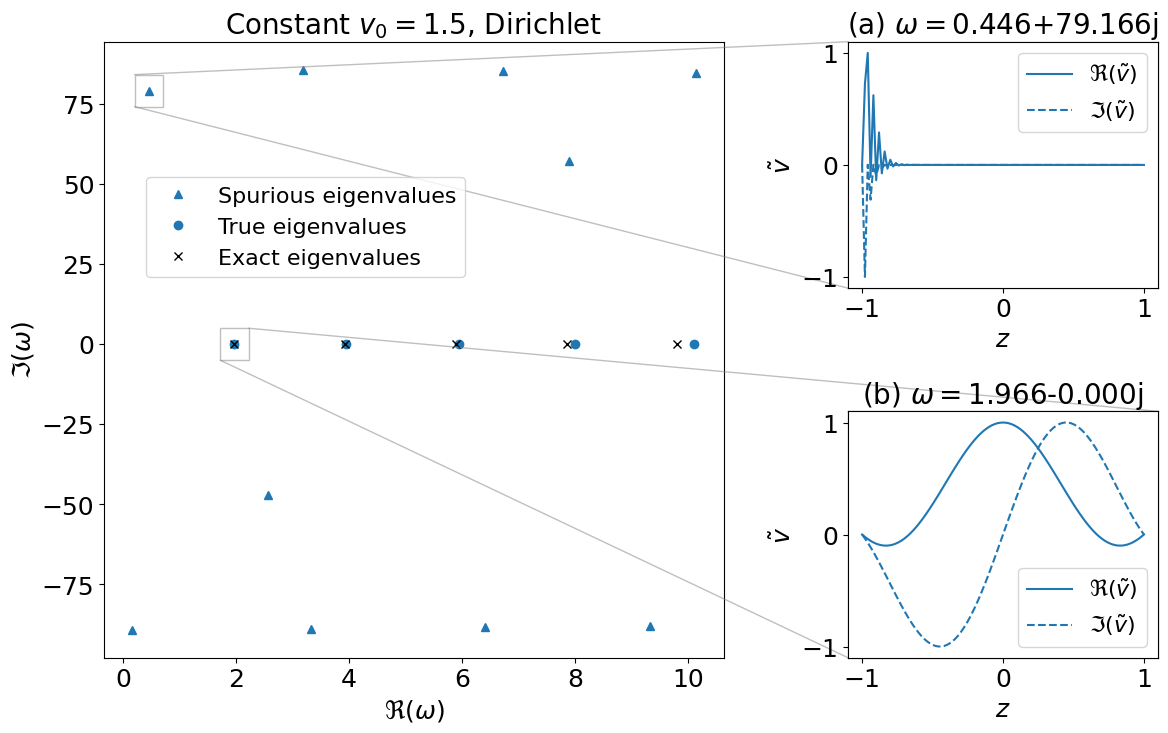
\includegraphics[width=\textwidth]{figures/eigenmodes-FD.png}
	\caption{(a) Eigenfunction corresponding to a spurious eigenvalue, the eigenfunction has weird shape. (b) Eigenfunction corresponding to a true eigenvalue.}
	\label{fig:eigenmodes-FD}
\end{figure}

In this simple case of solving Eq.~(\ref{eq:discretized-eq-G}), one way to filter the spurious modes is to remove modes with high-oscillation. That is removing modes with wave number $k>h/2 \arcsin(1/v_0)$. However, this is not possible in general cases because Eq.~(\ref{eq:dispersion-relation-G}) is only valid if finite-difference is used, and it requires the exact solution to the discretized problem Eq.~(\ref{eq:discretized-eq-G}) which is not available for non-constant velocity profile.

\subsection{Convergence Test}
To filter the spurious modes is by doing a "convergence test". Since the frequency Eq.~(\ref{eq:dispersion-relation-G}) is changing with mesh resolution $h$. From Fig.~\ref{fig:convergence-test} we see that only the true eigenmodes converge while the eigenvalues of spurious eigenmodes changes dramatically under different resolutions. By simply solving the discretized problem using spectral method under different mesh resolution, we can pick up the true eigenmodes by observing their convergence, and filter out the spurious eigenmodes which change dramatically with varying resolution.

\begin{figure} [htbp]
	\centering
	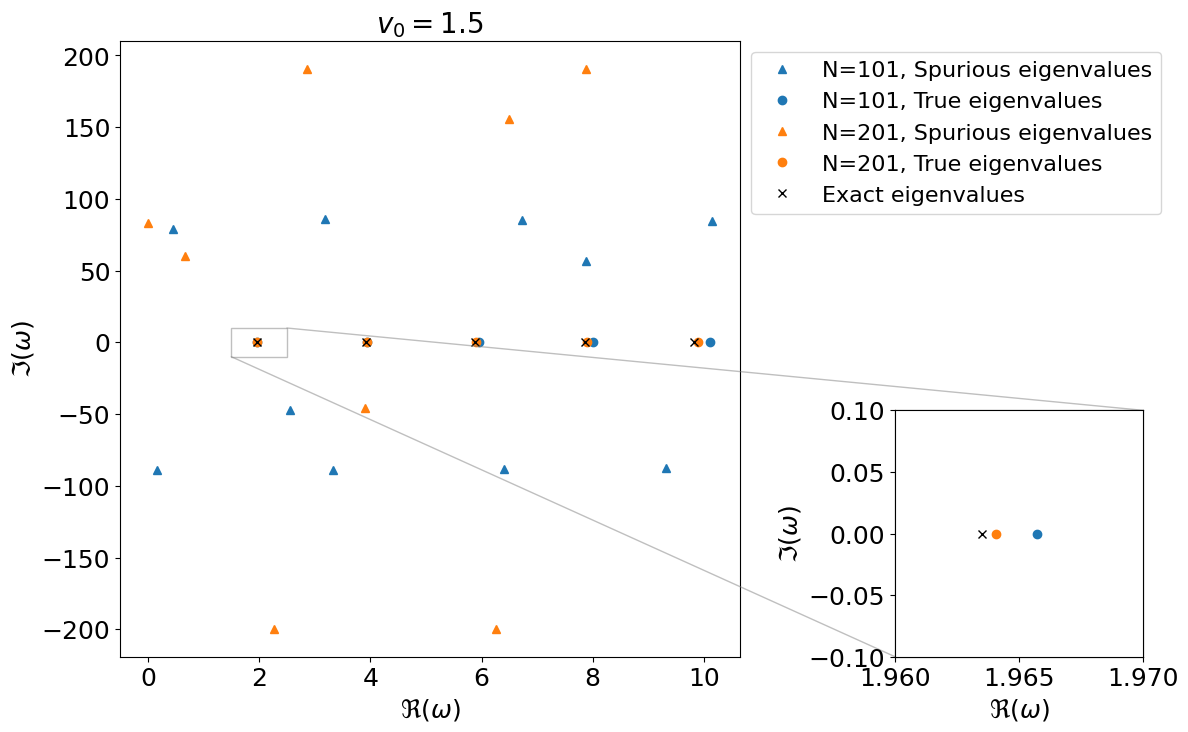
\includegraphics[width=\textwidth]{figures/convergence-test.png}
	\caption{The figure shows eigenvalues under different resolutions. True eigenvalues converge to the analytical eigenvalues as resolution increases. Spurious eigenvalues diverges with no obvious pattern.}
	\label{fig:convergence-test}
\end{figure}

\section{Plasma Flow with Constant Velocity Profile}
In this section, we will compute the eigenmodes of the constant velocity problem, Eq.~(\ref{eq:constant-v-problem}), with Dirichlet boundaries and the same problem with fixed-open boundaries, using spectral methods. More specifically, spectral-collocation and spectral-Galerkin methods will be employed. Then spurious modes will be filtered using the convergence test prescribed in previous section. Since we have already derived the exact solutions for the constant velocity cases in Sec.~\ref{sec:analytical-solutions}, we can ensure the accuracy and reliability of the numerical methods by comparing the numerical results to the analytical ones. The parameters of spectral methods are summarized in Table.~(\ref{table:parameters}). For spectral-collocation method, we use 101 points, and for spectral-Galerkin method we use 101 points and 30 basis functions.

\begin{table} [htbp]
	\centering
	\caption{With Dirichlet boundary condition, all methods have good accuracy, so using 101 nodes in the region $[0,1]$ is enough. For FE and SE methods, we use 50 basis functions.}
	\begin{tabular}{|c|c|c|}
		\hline
		                              & Collocation & Galerkin \\
		\hline
		M (number of points)          & 101         & 101      \\
		\hline
		N (number of basis functions) &             & 30       \\
		\hline
	\end{tabular}
	\label{table:parameters}
\end{table}

\subsection{Constant Subsonic Velocity Case}
Eq.~(\ref{eq:constant-v-problem}) is a special case of a more general polynomial eigenvalue problem Eq.~(\ref{eq:polynomial-eigenvalue-problem}). The existence of the exact solution allows us to verify the correctness of each method's implementation. This also serves as a reference to the accuracy spectral methods can achieve.

In summary, the plasma flow constant subsonic velocity profile is stable in the magnetic nozzle under both boundary conditions, Dirichlet boundary and fixed-open boundary. If the velocity is supersonic, then the plasma flow is stable is the boundary is Dirichlet, and is unstable if the boundary is fixed-open.

\subsubsection*{Dirichlet Boundary}
\begin{table} [htpb!]
	\centering
	\caption{Relative errors of first five eigenvalues obtained by spectral methods in constant subsonic velocity case with Dirichlet boundary condition. Numerical results agree with exact solution well.}
	\begin{tabular}{|c|c|c|c|c|c|}
		\hline
		$v_0=0.5$   & $\omega_1$     & $\omega_2$     & $\omega_3$     & $\omega_4$     & $\omega_5$     \\
		\hline
		Collocation & 3.48944421e-14 & 6.72512513e-14 & 1.59603736e-14 & 9.81718764e-15 & 4.07098462e-15 \\
		\hline
		Galerkin    & 4.09596742e-14 & 1.65697986e-14 & 4.97650778e-14 & 3.27344763e-13 & 4.11444935e-12 \\
		\hline
	\end{tabular}
	\label{table:eigenvalue-error-constant-subsonic-dirichlet}
\end{table}

\begin{figure}[htpb!]
	\centering
	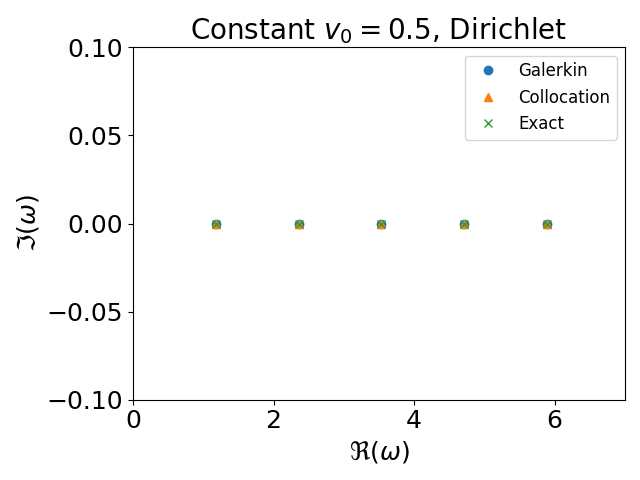
\includegraphics[width=0.7\linewidth]{figures/constant-subsonic-dirichlet.png}
	\caption{Showing the first five eigenvalues obtained by spectral-collocation and spectral-Galerkin methods. The plasma flow in the magnetic nozzle with constant subsonic velocity and Dirichlet boundary is stable. Spectral methods agree with exact eigenvalues.}
	\label{fig:constant-subsonic-dirichlet}
\end{figure}

Fig.~\ref{fig:constant-subsonic-dirichlet} shows that the eigenvalues obtained by spectral methods agree with the theoretical eigenvalues. Table.~\ref{table:eigenvalue-error-constant-subsonic-dirichlet} shows us the relative error $\abs{\omega_{numeric} - \omega_{analytic}}/\abs{\omega_{analytic}}$ is about $10^{-14}$ for each eigenvalue. Spectral methods indeed have high accuracy. Since the eigenvalues have almost zero imaginary parts, we consider the plasma flow with constant subsonic velocity in the magnetic nozzle with Dirichlet boundary is stable.


\subsubsection*{Fixed-Open Boundary}
\begin{table} [htbp!]
	\centering
	\caption{Relative error of each eigenvalue. Notice that the mode index starts from 0. These results agree with theory.}
	\begin{tabular}{|c|c|c|c|c|c|}
		\hline
		$v_0=0.5$   & $\omega_0$     & $\omega_1$     & $\omega_2$     & $\omega_3$     & $\omega_4$     \\
		\hline
		Collocation & 2.36006260e-12 & 1.95269435e-13 & 6.78183927e-14 & 2.43078107e-14 & 4.17011610e-14 \\
		\hline
		Galerkin    & 2.52491323e-12 & 2.19414097e-13 & 1.82417919e-13 & 5.92948284e-13 & 4.41481039e-12 \\
		\hline
	\end{tabular}
	\label{table:eigenvalue-error-fixed-open-subsonic}
\end{table}

\begin{figure}[htbp!]
	\centering
	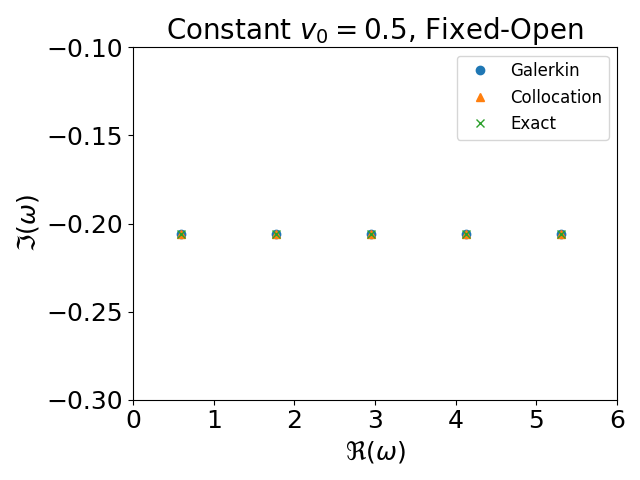
\includegraphics[width=0.7\linewidth]{figures/constant-subsonic-fixed-open.png}
	\caption{Showing the first five eigenvalues obtained by spectral-collocation and spectral-Galerkin methods. The plasma flow in the magnetic nozzle with constant subsonic velocity and fixed-open boundary is stable. Spectral methods agree with exact eigenvalues.}
	\label{fig:constant-subsonic-fixed-open}
\end{figure}

As shown in Fig.~\ref{fig:constant-subsonic-fixed-open} and Table.~\ref{table:eigenvalue-error-fixed-open-subsonic}, the numerical eigenvalues obtained by the spectral methods agree with the analytical eigenvalues. The relative errors $\abs{\omega_{numeric} -\omega_{analytic}}/\abs{\omega_{analytic}}$ are about $10^{-13}$. Again both spectral methods show good accuracy. Because the eigenvalues have negative imaginary parts, meaning the perturbations will exponential decay, so the plasma flow with constant subsonic velocity in the magnetic nozzle with fixed-open boundary is stable.

\subsection{Constant Supersonic Velocity Case}
In supersonic case, as predicted by Sec.~\ref{sec:analysis-of-numerical-spectrum}, spurious modes occur. Convergence test was used to filter the spurious modes.

\subsubsection*{Dirichlet Boundary}
\begin{table} [htbp!]
	\centering
	\caption{Relative error of first five filtered eigenvalues obtained by spectral methods in constant subsonic case under Dirichlet boundary. Numerical results agree with the theory, but we see the accuracy of eigenvalues obtained from spectral-Galerkin method drops after the 3rd one.}
	\begin{tabular}{|c|c|c|c|c|c|}
		\hline
		$v_0=1.5$   & $\omega_1$     & $\omega_2$     & $\omega_3$     & $\omega_4$     & $\omega_5$     \\
		\hline
		Collocation & 2.08984845e-13 & 9.29501612e-14 & 4.24537846e-14 & 3.38103217e-14 & 1.74476052e-14 \\
		\hline
		Galerkin    & 1.64805562e-13 & 6.09485884e-14 & 6.81795167e-12 & 1.95656738e-09 & 1.54134402e-07 \\
		\hline
	\end{tabular}
	\label{table:eigenvalue-error-dirichlet-supersonic}
\end{table}

\begin{figure}[htbp!]
	\centering
	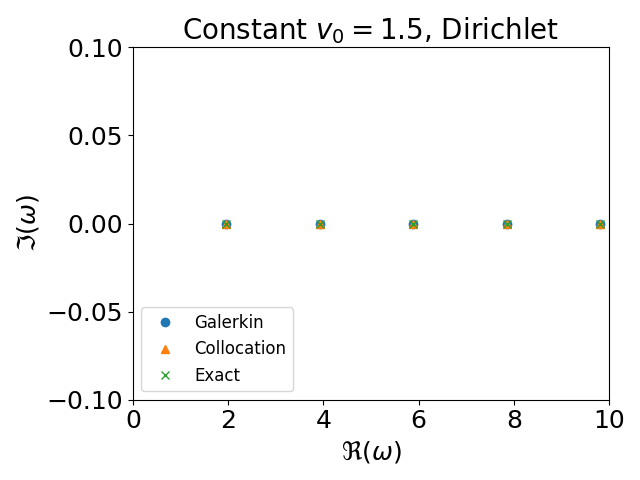
\includegraphics[width=0.7\linewidth]{figures/constant-supersonic-dirichlet.png}
	\caption{Showing the first five true eigenvalues obtained by spectral-collocation and spectral-Galerkin methods. The plasma flow in the magnetic nozzle with constant supersonic velocity and Dirichlet boundary is stable. Spectral methods agree with exact eigenvalues.}
	\label{fig:constant-supersonic-dirichlet}
\end{figure}

The first five filtered eigenvalues obtained by the two spectral methods are shown in Fig.~\ref{fig:constant-subsonic-dirichlet} and Table.~\ref{table:eigenvalue-error-dirichlet-supersonic} shows us the relative error of each of them compare to the corresponding exact eigenvalues. Good agreement between the spectral methods and the theoretical eigenvalues is shown. However, we see that the accuracy of spectral-Galerkin method drops for larger eigenvalues. The plasma flow with constant supersonic velocity is stable in the magnetic nozzle with Dirichlet boundary.

\subsubsection*{Fixed-Open Boundary}
\begin{table} [htbp!]
	\centering
	\caption{Relative error of first five eigenvalues obtained by spectral methods in constant supersonic case under fixed-open boundary. Results agree with theory. The accuracy of spectral-Galerkin method drops after first few eigenvalues.}
	\begin{tabular}{|c|c|c|c|c|c|}
		\hline
		$v_0=1.5$   & $\omega_0$     & $\omega_1$     & $\omega_2$     & $\omega_3$     & $\omega_4$     \\
		\hline
		Collocation & 5.10516649e-11 & 3.58709292e-12 & 8.72529437e-13 & 3.24263319e-13 & 1.34297439e-13 \\
		\hline
		Galerkin    & 5.38682371e-11 & 4.31902441e-12 & 1.44799870e-12 & 8.02395621e-11 & 2.05280524e-09 \\
		\hline
	\end{tabular}
	\label{table:eigenvalue-error-fixed-open-supersonic}
\end{table}

\begin{figure}[htbp!]
	\centering
	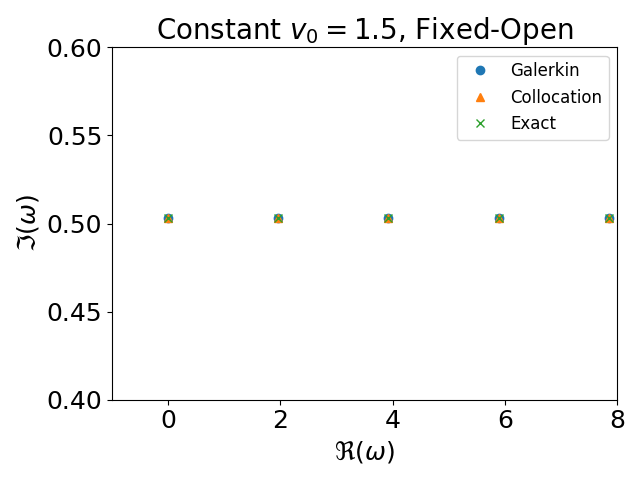
\includegraphics[width=0.7\linewidth]{figures/constant-supersonic-fixed-open.png}
	\caption{Showing the first five true eigenvalues obtained by spectral-collocation and spectral-Galerkin methods. The plasma flow in the magnetic nozzle with constant supersonic velocity and fixed-open boundary is unstable.}
	\label{fig:constant-supersonic-fixed-open}
\end{figure}

Table.~\ref{table:eigenvalue-error-fixed-open-supersonic} shows relative error for the first five filtered eigenvalues obtained by different spectral methods. We see that the accuracy of spectral-Galerkin method drops for larger eigenvalues. Fig.~\ref{fig:constant-supersonic-fixed-open} shows us that plasma flow with constant supersonic velocity is unstable in the magnetic nozzle with fixed-open boundary.

\section{Plasma Flow with Spatial Varying Velocity Profiles}
In previous section we have already verify the accuracy of spectral methods by comparing the numerical results to the analytical solutions to the eigenvalue problem with constant velocity plasma flow, Eq.~(\ref{eq:constant-v-problem}). In this section we will apply spectral methods to the eigenvalue problem with spatial varying velocity profiles. That is Eq.~(\ref{eq:polynomial-eigenvalue-problem}) with Dirichlet boundary and fixed-open boundary conditions. The parameters for spectral methods are the same as Table.~\ref{table:parameters}.

\subsection{Subsonic Case}
In this case, the plasma flows with subsonic velocity. The velocity profile is spatial varying and will reach its maximum $0.5$ Mach at the nozzle throat $z=0$. The velocity profile is the orange line shown in Fig.~\ref{fig:velocity-profiles}. When applying spectral methods, no spurious modes were found in subsonic case. Similar to the case with constant velocity profile, we experiment with two boundary conditions: Dirichlet boundary and fixed-open boundary. We found that the plasma flow is stable when the boundary condition is Dirichlet and is stable (except ground mode) when using fixed-open boundary.

\subsubsection*{Dirichlet Boundary}
\begin{figure} [htbp!]
	\centering
	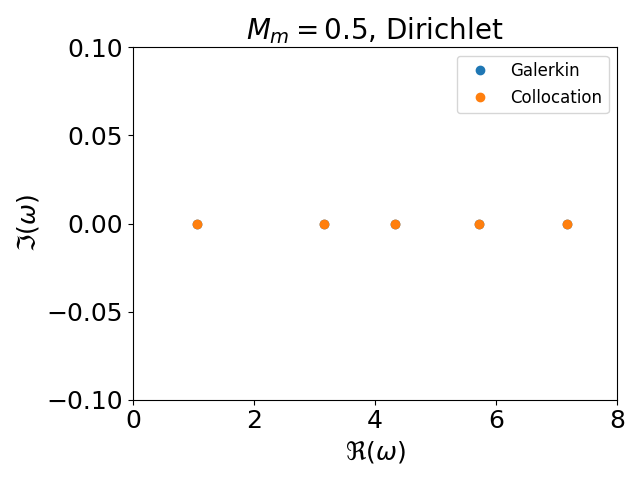
\includegraphics[width=0.7\linewidth]{figures/subsonic-drichlet.png}
	\caption{Showing the first five eigenvalues obtained by spectral-collocation and spectral-Galerkin method. This indicates that the subsonic plasma flow in magnetic nozzle with Dirichlet boundary is stable. Two methods agree with each other well enough the eigenvalues are overlapped.}
	\label{fig:subsonic-dirichlet}
\end{figure}
With Dirichlet boundary condition, $\tilde{v}(\pm 1) =0$, the subsonic plasma flow in magnetic nozzle is stable. Fig.~\ref{fig:subsonic-dirichlet} shows the first five eigenvalues obtained by different spectral methods. The two methods, spectral-collocation and spectral-Galerkin, agree with each other well enough so the eigenvalues are overlapped on the figure. These eigenvalues has zero imaginary parts (to be more specific, $\abs{\Im{\omega}} < 10^{-13}$), meaning that the subsonic plasma flow in the magnetic nozzle is stable.

\subsubsection*{Fixed-Open Boundary}
\begin{figure} [htbp!]
	\centering
	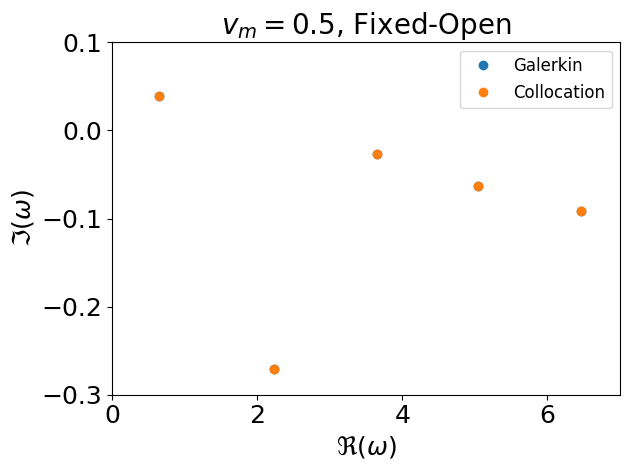
\includegraphics[width=0.7\linewidth]{figures/subsonic-fixed-open.png}
	\caption{Showing the first five eigenvalues obtained by spectral-collocation and spectral-Galerkin method. This indicates that the subsonic plasma flow in magnetic nozzle with fixed-open boundary is stable (except ground mode). Two methods agree with each other well enough the eigenvalues are overlapped.}
	\label{fig:subsonic-fixed-open}
\end{figure}
Fig.~\ref{fig:subsonic-fixed-open} shows the first five eigenvalues obtained by the two spectral methods. The results agree with each other well enough so the eigenvalues are overlapped. We see that the eigenvalues have negative imaginary parts (except ground mode), indicating that the subsonic plasma flow in the nozzle with fixed-open boundary is stable (except ground mode).

\subsection{Supersonic Case}
In this subsection, we are going to investigate the instability of supersonic plasma flow in the magnetic nozzle. The velocity profile is the purple line shown in Fig.~\ref{fig:velocity-profiles}. The plasma flow reaches its minimum velocity $1.5$ Mach at the nozzle throat $z=0$. When applying spectral methods, spurious modes occur and we need to apply convergence test to extract the true eigenvalues. We found that the supersonic plasma flow is stable when the Dirichlet boundary condition was used, and is unstable the boundary is fixed-open.

\subsubsection*{Dirichlet Boundary}
\begin{figure} [htbp!]
	\centering
	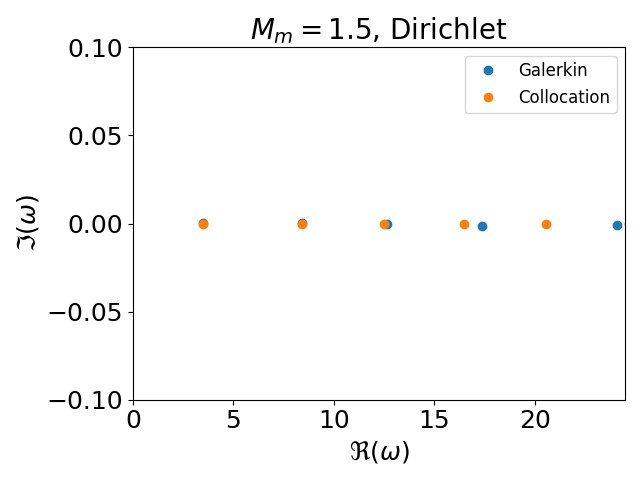
\includegraphics[width=0.7\linewidth]{figures/supersonic-drichlet.png}
	\caption{Showing the first five true eigenvalues obtained by spectral-collocation and spectral-Galerkin method. This indicates that the supersonic plasma flow in magnetic nozzle with Dirichlet boundary is stable. Two methods agree well on the first 3 eigenmodes, and starts to deviate from each other after that. Nevertheless, these eigenvalues have near-zero imaginary parts. The eigenvalues obtained by spectral-Galerkin have imaginary parts within $\pm10^{-3}$ and the eigenvalues obtained by spectral-collocation have imaginary parts within $\pm10^{-13}$.}
	\label{fig:supersonic-dirichlet}
\end{figure}
As shown Fig.~\ref{fig:supersonic-dirichlet}, the two spectral methods agree well on the first three eigenvalues but starts to have noticeable difference afterward. Despite having different real parts in the eigenvalues, these eigenvalues all have near-zero imaginary parts. The imaginary parts of the eigenvalues obtained by spectral-collocation method are within $\pm10^{-13}$, and the imaginary parts of the eigenvalues obtained by spectral-Galerkin method are within $\pm10^{-3}$. This suggests the supersonic plasma flow in the magnetic nozzle with Dirichlet boundary is stable.

\subsubsection*{Fixed-Open Boundary}
\begin{figure} [htbp!]
	\centering
	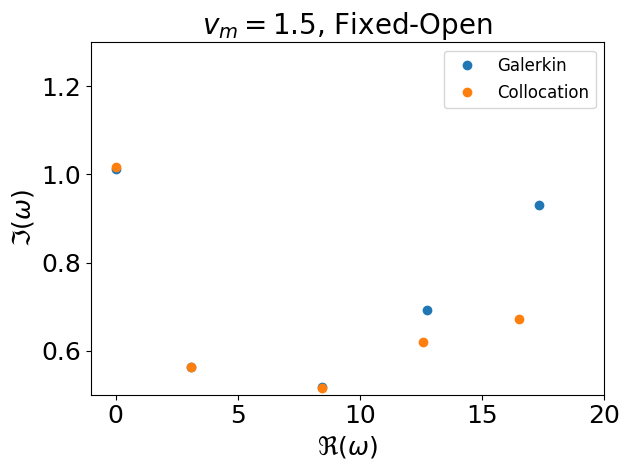
\includegraphics[width=0.7\linewidth]{figures/supersonic-fixed-open.png}
	\caption{Showing the first five true eigenvalues obtained by spectral-collocation and spectral-Galerkin method. Two methods agree well on the first three modes, and start to have significant difference after that. Despite having some different eigenvalues, these eigenvalues all have positive imaginary parts, suggesting that the supersonic plasma flow in the magnetic nozzle with fixed-open boundary is unstable.}
	\label{fig:supersonic-fixed-open}
\end{figure}
In Fig.~\ref{fig:supersonic-fixed-open}, we see that the two spectral methods agree well on the first three eigenvalues but starts to have noticeable difference afterward. Despite having different eigenvalues after the third eigenvalue, these eigenvalues all have positive imaginary parts, suggesting the supersonic plasma flow in the magnetic nozzle with fixed-open boundary is unstable.

\chapter{Singular Perturbation} \label{chap:singular-perturbation}
When dealing with the accelerating velocity profile, spectral methods struggle to yield meaningful results because of the singularity at the nozzle throat ($z=0$). This chapter is dedicated to analyze the polynomial eigenvalue problem with transonic velocity profile. We start by showing the existence of the singularity of Eq.~(\ref{eq:polynomial-eigenvalue-problem}), and how spectral methods introduced in previous chapter failed to resovle solutions. Then we will discuss the concept of singular perturbation and will pickup regular solutions to Eq.~(\ref{eq:polynomial-eigenvalue-problem}) near the nozzle throat $z=0$ using Frobenius method. Finally, we will introduce shooting method and use it together with the regular solutions to find eigenmodes.

\section{Presence of Singularity in Transonic cases} \label{sec:presence-of-singularity}
In order to see the existence of the singularity, we rearrange the terms the polynomial eigenvalue problem, Eq.~(\ref{eq:polynomial-eigenvalue-problem}),
\begin{equation} \label{eq:singular-perturbation-problem}
	\begin{aligned}
		  & (1-v_0^2)\pdv[2]{\tilde{v}}{z}                                                                                                                                        \\
		+ & \left[2i\omega v_0 - \left(3v_0 + \frac{1}{v_0}\right)\pdv{v_0}{z}\right]\pdv{\tilde{v}}{z}                                                                           \\
		+ & \left[\omega^2 + 2i\omega\pdv{v_0}{z} -\left(1 - \frac{1}{v_0^2}\right)\left(\pdv{v_0}{z}\right)^2 - \left(v_0 + \frac{1}{v_0}\right)\pdv[2]{v_0}{z} \right]\tilde{v} \\
		= & 0
	\end{aligned}
\end{equation}
This is a second order ordinary differential equation defined on region $[-1,1]$.

For transonic (accelerating and decelerating) velocity profiles (Fig.~\ref{fig:velocity-profiles}), the plasma flow is at sonic point at the throat of the nozzle, $v_0(0)=1$. Therefore, the highest order term vanishes at $z=0$. It is a singular point, and it is the  cause of the failure of spectral method, see Fig.~(\ref{fig:failure-of-spectral-method}). Spectral method is unable to resolve meaningful eigenfunctions, the eigenfunctions are squeezed together at $z=0$, hence resulting wrong eigenvalues.

\begin{figure} [htbp]
	\centering
	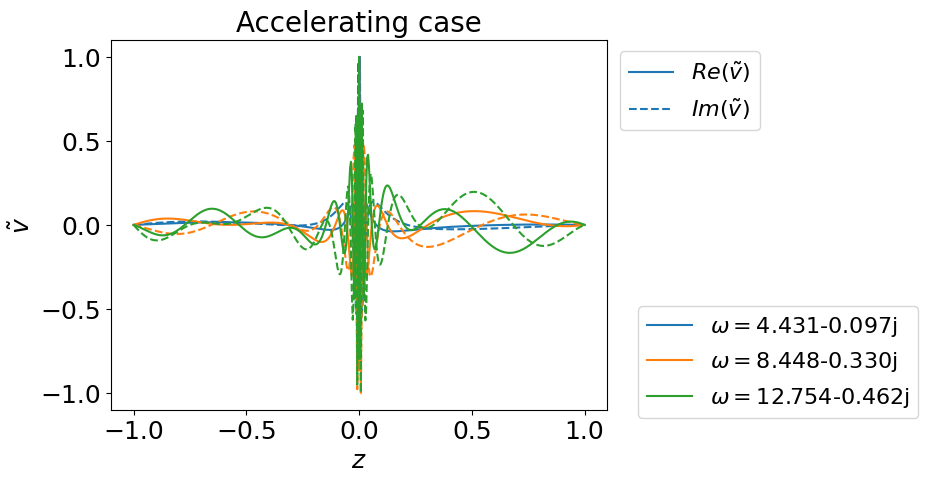
\includegraphics[width=0.7\textwidth]{figures/results-bad-accelerating-v}
	\caption{An attempt to solve the polynomial eigenvalue problem, Eq.~(\ref{eq:polynomial-eigenvalue-problem}) using finite-difference. Eigenfunctions are squeezed to the center of the nozzle due to the existence of the singularity at $z=0$.}
	\label{fig:failure-of-spectral-method}
\end{figure}

\section{Expansion at Singularity}
In this section, we will try to extract the regular solutions to Eq.~(\ref{eq:singular-perturbation-problem}) using Frobenius method. It is speculated such regular solutions exist. Further analysis and numerical simulations also validate the existence of such solutions. In order to find them, we need to expand terms in Eq.~(\ref{eq:singular-perturbation-problem}) about the singularity.

The first task is to linearize the terms with $v_0$ about the singularity. The linearization of $v_0(z) = 1 + v_0'(0)z$ is a good approximation to the original function $v_0(z)$ because the transonic velocity profiles are linear in the neighborhood of $z=0$, as we can see from Fig.~\ref{fig:velocity-profiles}. Therefore, through some simple algebra we obtain,
\begin{equation}
	\begin{aligned}
		1-v_0^2              & = -2v_0'(0)z    \\
		3v_0 + \frac{1}{v_0} & = 4 + 2v_0'(0)z \\
		1-\frac{1}{v_0^2}    & = 2v_0'(0)z     \\
		v_0 + \frac{1}{v_0}  & = 2
	\end{aligned}
\end{equation}

Then Eq.~(\ref{eq:singular-perturbation-problem}) becomes
\begin{equation} \label{eq:perturbed-equation-full}
	\begin{aligned}
		- & 2v_0'(0)z\pdv[2]{\tilde{v}}{z}                                              \\
		+ & [2i\omega - 4v_0'(0) + (2i\omega - 2v_0'(0))z]\pdv{\tilde{v}}{z}            \\
		+ & \left[\omega^2 + 2i\omega v_0'(0) - 2v_0''(0) - 2v_0'(0)^3z\right]\tilde{v}
		= 0
	\end{aligned}
\end{equation}

In fact, we can further simply the equation by dropping all $z$ terms except the first term (second-order derivative term). It can be shown that dropping the $z$ terms except the second derivative in Eq.~(\ref{eq:perturbed-equation-full}) does not affect the first order correction ($\tilde{v}$ is the same up to $z$ term), it is an acceptable approximation.
\begin{equation}
	- 2v_0'(0)z\pdv[2]{\tilde{v}}{z}
	+ (2i\omega - 4v_0'(0))\pdv{\tilde{v}}{z}
	+ (\omega^2 + 2i\omega v_0'(0) - 2v_0''(0))\tilde{v}
	= 0
\end{equation}

Dividing by the first coefficient, we have
\begin{equation}
	z\pdv[2]{\tilde{v}}{z} + a\pdv{\tilde{v}}{z} + b\tilde{v} = 0
	\label{eq:perturbed-equation}
\end{equation}
where
\begin{equation}
	a = \frac{2i\omega - 4v_0'(0)}{-2v_0'(0)}; \quad
	b = \frac{\omega^2 + 2i\omega v_0'(0) - 2v_0''(0)}{-2v_0'(0)}
\end{equation}

Use Frobenius method, we assume the velocity perturbation can be written as a power series in $z$,  $\tilde{v} = \sum_{n\geq 0}c_nz^{n+r}$. By substituting the power series into Eq.~(\ref{eq:perturbed-equation}) we have
\begin{equation}
	\sum_{n \geq 0} (n+r)(n+r+1) c_n z^{n+r-1} + a(n+r)c_nz^{n+r-1} + bc_nz^{n+r} = 0
\end{equation}
Shift the power of the last term we get
\begin{equation}
	\sum_{n \geq 0} (n+r)(n+r+1) c_n z^{n+r-1} + a(n+r)c_nz^{n+r-1} + \sum_{n \geq 1} bc_{n-1}z^{n+r-1} = 0
\end{equation}

Setting $n=0$, we get the indicial equation
\begin{equation}
	c_0 r(r-1) + c_0 ar = 0 \Rightarrow c_0r(r+a-1) = 0
\end{equation}
We get two different roots, $r=0$ and $r=1-a$. They correspond to finite solution and diverging solution near the singularity, respectively.

The coefficients are given by recurrence relation
\begin{equation}
	(n+r)(n+r-1)c_n + a(n+r)c_n + bc_{n-1} = 0
	\Rightarrow
	c_n = \frac{-bc_{n-1}}{(n+r)(n+r-1+a)}
\end{equation}
Solving this relation we get explicit expression for $c_n$, $n\in\mathbb{N}$,
\begin{equation}
	\begin{aligned}
		c_n & = \frac{(-1)^n b^n c_0}{\prod_{k=0}^{n-1} (n+r-k)(n+r-1+a-k)}              \\
		    & = (-1)^n b^n c_0 \frac{\Gamma(r+1)\Gamma(r+a)}{\Gamma(n+r+1)\Gamma(n+r+a)}
	\end{aligned}
	\label{eq:coefficient}
\end{equation}

Therefore, we successfully extracted the regular solution (corresponding to the root $r=0$) in the form of power series,
\begin{equation} \label{eq:regular-solution}
	\begin{aligned}
		\tilde{v} & = c_0 + c_1z + c_2z^2 + \cdots                               \\
		          & = c_0 - c_0\frac{b}{a}z + c_0\frac{b^2}{2a(1+a)}z^2 + \cdots
	\end{aligned}
\end{equation}

It is worth to mention that the diverging solution (corresponding to the root $r=a$) goes like
\begin{equation}
	\tilde{v}(z) \sim z^{1-a} = z^{-1-\omega_i/v_0'(0)}z^{i\omega_r/v_0'(0)}
\end{equation}
where $\omega = \omega_r + i\omega_i$. Meaning that the divergent solution will start to diverge when $\omega_i > -v'(0)$.

\section{Shooting Method}
The existence of divergent solutions makes the problem hard to solve numerically using spectral method. One workaround involves manually selecting regular solutions during the numerical process. The shooting method, a suitable numerical technique, is capable of incorporating information of regular solutions. In other words, $\tilde{v}$ and its derivatives at the nozzle throat $z=0$ can be incorporate into the numerical process. Due to this restriction of singularity, we are not allowed to impose any boundary condition at the nozzle exit, $z=1$, anymore because the information of the regular solution already serve as a boundary condition.

Our polynomial eigenvalue problem, Eq.~(\ref{eq:polynomial-eigenvalue-problem}), can be formulated in the following form,
\begin{equation}
	f(z, \tilde{v}, \tilde{v}', \tilde{v}''; \omega) = 0
	\quad
	-1\leq z \leq 0,
	\quad
	\tilde{v}(-1) = 0, \tilde{v}(0) = 1
\end{equation}
where $f$ is the function defined on the left of equal sign of Eq.~(\ref{eq:polynomial-eigenvalue-problem}). The task for shooting method is to find eigenvalues $\omega$ and their corresponding eigenfunctions $\tilde{v}$ such that $f=0$ holds. Meanwhile, the eigenfunctions must satisfy the boundary conditions at the entrance $z=-1$ and at the throat $z=0$. After obtaining the solutions, we can extend the solution to $z=1$. The extension is unique, more details will be explained later.

However, to make the formulation more suitable for numerical computation, we would like to rewrite the second differential equation as two first order differential equations,
\begin{equation}
	\dv{z}\mathbf{\tilde{u}} = \mathbf{f}(\mathbf{\tilde{u}},z;\omega),
	\quad
	-1 \leq z \leq 0,
	\quad
	\tilde{v}(-1) = 0, \tilde{v}(0) = 1
	\label{eq:shooting-method-formulation}
\end{equation}
Let $\mathbf{\tilde{u}} = [\tilde{v}, \tilde{u}]^T$, the polynomial eigenvalue problem is transformed to
\begin{align*}
	\tilde{v}' & = \tilde{u}                \\
	\tilde{u}' & = \frac{-1}{1-v_0^2}\left[
		\omega^2\tilde{v} + 2i\omega(v_0+v_0'\tilde{v}) - \left(3v_0 - \frac{1}{v_0}\right)v_0'\tilde{u} - \left(1-\frac{1}{v_0}^2\right)(v_0')^2\tilde{v} - \left(v_0+\frac{1}{v_0}v_0''\tilde{v}\right)
	\right]                                 \\
\end{align*}
together with two boundary conditions, $\tilde{v}(-1) = 0$ and $\tilde{v}(0) = 1$. The task of shooting method remains the same: find $\mathbf{\tilde{u}}$ and $\omega$ such that $\dv*{\mathbf{\tilde{u}}}{z} = \mathbf{f}$ and $\tilde{v}$ must satisfy the boundary conditions.

Suppose $\omega$ is given. We can find $\mathbf{\tilde{u}}(-1)$, and hence $\tilde{v}(-1)$ by applying 4th order Runge-Kutta method (RK4) to the following IVP,
\begin{equation}
	\dv{z}\mathbf{\tilde{u}} = \mathbf{f}(\mathbf{\tilde{u}},z;\omega), \quad
	-1 \leq z \leq 0, \quad
	\mathbf{\tilde{u}}(0)=\mqty[\tilde{v}(0) \\ \tilde{u}(0)], \dv{z}\mathbf{\tilde{u}}(0) =\mqty[\tilde{v}'(0) \\ \tilde{u}'(0)]
	\label{eq:shooting-method-ivp}
\end{equation}
The information of the regular solution is built into the numerical process by setting the initial conditions,
\begin{equation}
	\begin{aligned}
		\mathbf{\tilde{u}}       & = \mqty[\tilde{v}(0)  \\ \tilde{u}(0)]
		= \mqty[c_0                                      \\ c_1]
		= \mqty[1                                        \\ (2i\omega v_0'-2v_0'')/2v_0'] \\
		\dv{z}\mathbf{\tilde{u}} & = \mqty[\tilde{v}'(0) \\ \tilde{u}'(0)]
		= \mqty[\tilde{u}(0)                             \\ c_2]
		= \mqty[(2i\omega v_0'-2v_0'')/2v_0'             \\ -((v_0')^4+(2i\omega v_0' + (v_0')^2 - v_0'')(i\omega v_0' - v_0''))/(v_0'(2i\omega-6v_0'))]
	\end{aligned}
\end{equation}
The coefficients $c_0, c_1$, and $c_2$ are obtained from the power series expansion of $\tilde{v}$ near $z=0$, Eq.~(\ref{eq:regular-solution}).

The above step can be abstracted as a function, $h(\omega) = \tilde{v}(-1)$. This function takes in a variable $\omega$, and it spits out the value $\tilde{v}(-1)$ by applying RK4 to the I.V.P. Eq.~(\ref{eq:shooting-method-ivp}). We then apply root finding algorithm to this function $h$ to find $\omega$ such that $\tilde{v}$ satisfies the boundary condition at the entrance, $h(\omega)=\tilde{v}(-1)=0$. This process can be viewed as trying to land a projectile at certain location, i.e. $\tilde{v}(-1)=0$, by adjusting the shooting angle, i.e. $\omega$, hence the name shooting method.

After finding $\omega$, we can extend the numerical solution $\tilde{v}$ to the region $[0,1]$. We simply apply RK4 to the following I.V.P.
\begin{equation}
	\dv{z}\mathbf{\tilde{u}} = \mathbf{f}(\mathbf{\tilde{u}},z;\omega), \quad
	0 \leq z \leq 1, \quad
	\mathbf{\tilde{u}}(0)=\mqty[\tilde{v}(0) \\ \tilde{u}(0)], \dv{z}\mathbf{\tilde{u}}(0) =\mqty[\tilde{v}'(0) \\ \tilde{u}'(0)]
\end{equation}
Since $\omega$ is already found, the initial conditions are given. The function $\mathbf{f}$ is continuous in $z$ on $[0,1]$ and is Lipschitz in $\mathbf{\tilde{u}}$ due to the fact $\mathbf{f}$ is continuous on a compact region $[0,1]$. Hence, the solution to this I.V.P. exists and is unique.


\section{Plasma Flow with Accelerating Velocity Profile}
Starting from the singular point, we shoot the regular solution to the left boundary. We find the set of eigenvalues such that $\tilde{v}(-1)=0$. With these eigenvalues, we can extend the solution to the supersonic region $(0,1]$. The first few eigenmodes are drawn in Fig.~\ref{fig:results-accelerating-v}. The eigenmodes indicates that the accelerating plasma flow is stable.
\begin{figure} [H]
	\centering
	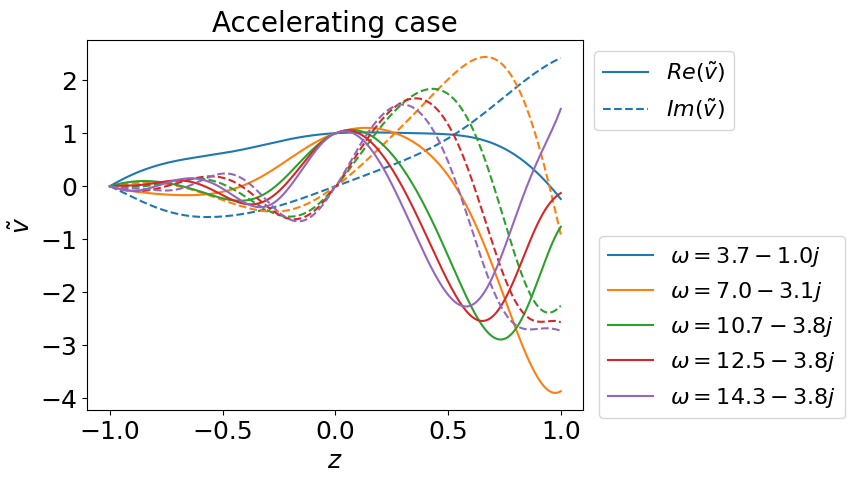
\includegraphics[width=0.7\linewidth]{figures/results-accelerating-v}
	\caption{Showing the first 5 eigenmodes, they are stable.}
	\label{fig:results-accelerating-v}
\end{figure}

\chapter{Numerical Experiments} \label{chap:numerical-experiments}
In this chapter, we will solve the eigenvalue problem, Eq.(\ref{eq:eigenvalue-problem}), with different discretizations. There will be three major categories of methods used. Finite difference (FD) method, finite element (FE) method and spectral element method (SE).

The finite difference method will be used together with equally spaced nodes. The finite element method will use B-spline as basis functions. Finally, the spectral element method uses sine functions as the spectral elements.

For Dirichlet boundary, The parameters of different discretizations are listed below
\begin{table} [H]
	\centering
	\caption{With Dirichlet boundary condition, all methods have good accuracy, so using 101 nodes in the region $[0,1]$ is enough. For FE and SE methods, they are using ~50 basis functions.}
	\begin{tabular}{|c|c|c|c|}
		\hline
		           & FD  & FE\_BSPLINE & SE\_SINE \\
		\hline
		N          & 101 & 101         & 101      \\
		\hline
		NUM\_BASIS &     & 51          & 50       \\
		\hline
	\end{tabular}
	\label{table:parameters-dirichlet}
\end{table}

For left-fixed and right-open (fixed-open) boundary condition, the parameters are
\begin{table} [H]
	\centering
	\caption{With fixed-open boundary condition, it requires higher resolution in order to get accurate results. Therefore all methods use 501 nodes in the region $[0,1]$, and FE method uses 101 basis functions.}
	\begin{tabular}{|c|c|c|}
		\hline
		           & FD  & FE\_BSPLINE \\
		\hline
		N          & 501 & 501         \\
		\hline
		NUM\_BASIS &     & 101         \\
		\hline
	\end{tabular}
	\label{table:parameters-fixed-open}
\end{table}


\section{Constant Velocity Case}
\subsection{Dirichlet Boundary}
Because the existence of exact solution to problems Eq.(\ref{eq:constant-v-problem-dirichlet}). The case with constant velocity profile is used as a sanity check. It allows us to verify the correctness of each method's implementation. This also serves as a reference to the accuracy spectral methods can achieve.

From Fig.(\ref{fig:constant-v-dirichlet}), we see that the order of growth rates obtained by different methods is about $~10^{-14}$ for both subsonic and supersonic cases. We will use these numbers as a reference to the accuracy of our numerical methods. If a method produces growth rates with order close to $10^{-14}$, we consider the growth rates to be 0.

\begin{table} [H]
	\centering
	\caption{Relative error of each eigenvalue.}
	\begin{tabular}{|c|c|c|c|c|c|}
		\hline
		$v_0=0.5$ & 1         & 2         & 3         & 4         & 5         \\
		\hline
		FD        & 2.827e-05 & 1.130e-04 & 2.541e-04 & 4.512e-04 & 7.040e-04 \\
		\hline
		FE        & 0.005     & 0.005     & 0.006     & 0.008     & 0.010     \\
		\hline
		SE        & 2.896e-05 & 1.157e-04 & 2.603e-04 & 4.626e-04 & 7.217e-04 \\
		\hline
	\end{tabular}
	\begin{tabular}{|c|c|c|c|c|c|}
		\hline
		$v_0=1.5$ & 1     & 2     & 3     & 4     & 5     \\
		\hline
		FD        & 0.001 & 0.005 & 0.010 & 0.019 & 0.030 \\
		\hline
		FE        & 0.006 & 0.010 & 0.019 & 0.029 & 0.043 \\
		\hline
		SE        & 0.001 & 0.005 & 0.011 & 0.019 & 0.030 \\
		\hline
	\end{tabular}
	\label{table:eigenvalue-error-dirichlet}
\end{table}

\begin{figure}[H]
	\centering
	\begin{subfigure}{0.5\textwidth}
		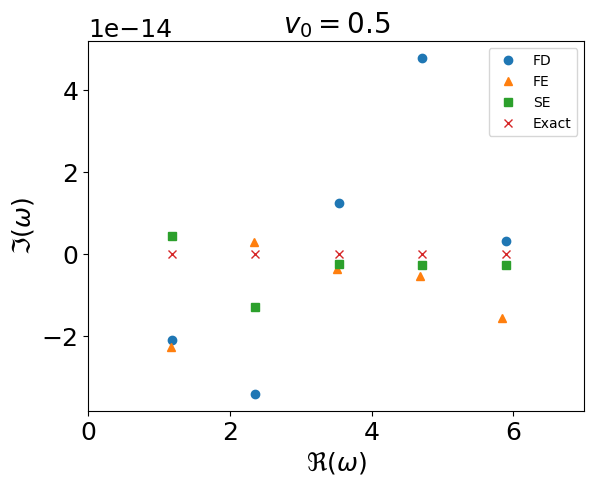
\includegraphics[width=\linewidth]{figures/fixed-fixed-constant-v-v0=0.5}
		\caption{All modes are stable.}
	\end{subfigure}%
	\begin{subfigure}{0.5\textwidth}
		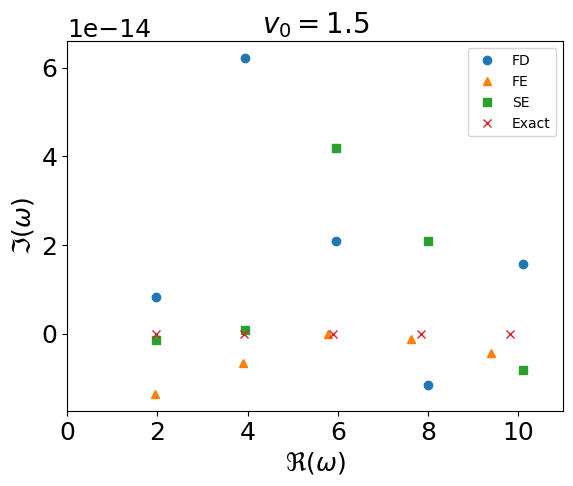
\includegraphics[width=\linewidth]{figures/fixed-fixed-constant-v-v0=1.5}
		\caption{Filtered modes are stable.}
	\end{subfigure}
	\caption{Showing the first 5 eigenvalues of each method in each case. All methods are close to the exact eigenvalues.}
	\label{fig:constant-v-dirichlet}
\end{figure}

\subsection{Fixed-Open Boundary}
\begin{table} [H]
	\centering
	\caption{Relative error of each eigenvalue. Notice that the ground mode for subsonic case is non-zero.}
	\begin{tabular}{|c|c|c|c|c|c|}
		\hline
		$v_0=0.5$ & 0         & 1         & 2         & 3         & 4         \\
		\hline
		FD        & 1.209e-05 & 3.458e-05 & 5.775e-05 & 8.153e-05 & 1.061e-04 \\
		\hline
		FE        & 8.090e-05 & 2.007e-04 & 2.981e-04 & 6.596e-04 & 1.821e-03 \\
		\hline
	\end{tabular}
	\begin{tabular}{|c|c|c|c|c|c|}
		\hline
		$v_0=1.5$ & 1         & 2         & 3         & 4         & 5         \\
		\hline
		FD        & 9.163e-05 & 2.435e-04 & 4.833e-04 & 8.160e-04 & 1.243e-03 \\
		\hline
		FE        & 4.431e-04 & 7.924e-04 & 1.516e-03 & 3.103e-03 & 8.001e-03 \\
		\hline
	\end{tabular}
	\label{table:eigenvalue-error}
\end{table}

\begin{figure}[H]
	\centering
	\begin{subfigure}{0.5\textwidth}
		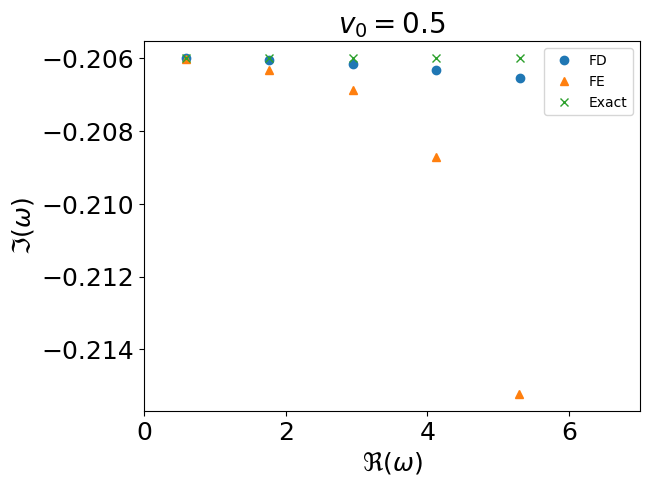
\includegraphics[width=\linewidth]{figures/fixed-open-constant-v-v0=0.5}
		\caption{All modes are stable.}
	\end{subfigure}%
	\begin{subfigure}{0.5\textwidth}
		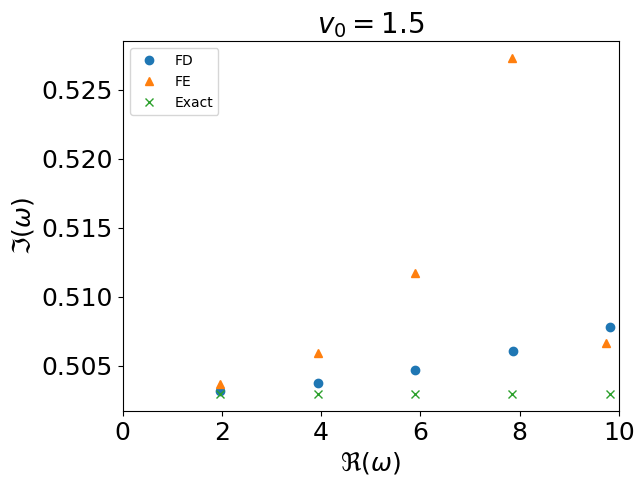
\includegraphics[width=\linewidth]{figures/fixed-open-constant-v-v0=1.5}
		\caption{All modes are unstable.}
	\end{subfigure}
	\caption{Showing the first 5 eigenvalues of each method. Finite-difference method has much better accuracy than finite-element method.}
	\label{fig:constant-v-fixed-open}
\end{figure}


\section{Subsonic Case}
\subsection{Dirichlet Boundary}
When setting the mid-point velocity to be $M_m=0.5$, we have the subsonic velocity profile. This velocity profile is the orange line shown in Fig.\ref{fig:velocity-profiles}. With Dirichlet boundary condition, $\tilde{v}(\pm 1) =0$. The flow in magnetic nozzle is stable. Fig.\ref{fig:subsonic-v-dirichlet} shows the first few eigenvalues obtained by different discretizations.

The order of growth rates obtained by different methods is $10^{-13}$, we can consider it to be stable.
\begin{figure} [H]
	\centering
	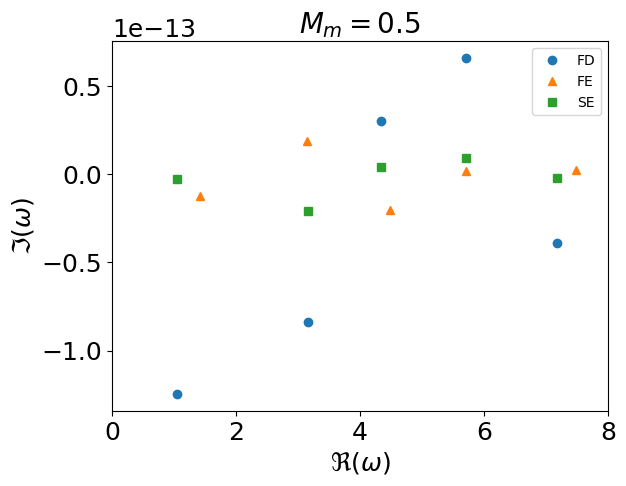
\includegraphics[width=0.7\linewidth]{figures/fixed-fixed-subsonic-v}
	\caption{Showing the first 5 modes. It suggests that the flow in magnetic nozzle with subsonic velocity profile and Dirichlet boundary condition is stable.}
	\label{fig:subsonic-v-dirichlet}
\end{figure}

\subsection{Fixed-Open Boundary}
\begin{figure} [H]
	\centering
	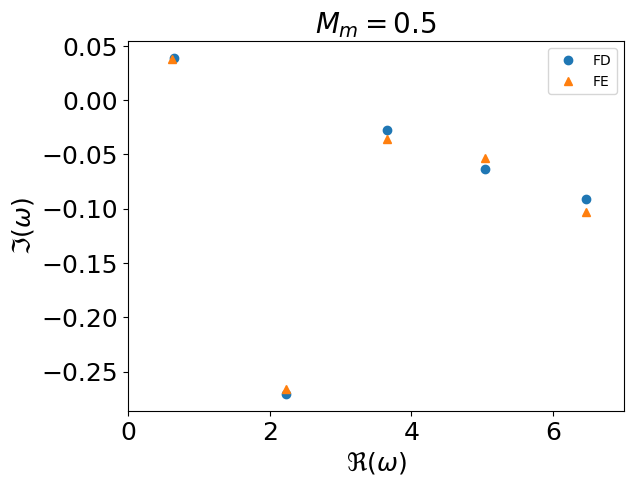
\includegraphics[width=0.7\linewidth]{figures/fixed-open-subsonic-v}
	\caption{Showing the first 5 modes. The ground mode is unstable, other modes are stable.}
	\label{fig:subsonic-v-fixed_open}
\end{figure}


\section{Supersonic Case}
\subsection{Dirichlet Boundary}
When the velocity profile is supersonic, shown as purple line in Fig.\ref{fig:velocity-profiles}, spurious modes appeared as predicted in Chap.\ref{chap:theoretical-analysis}. Using the convergence test, we successfully eliminates all unstable modes. Fig.(\ref{fig:supersonic-v-dirichlet}) shows the first few filtered eigenvalues. As we can see the flow is stable.
\begin{figure} [H]
	\centering
	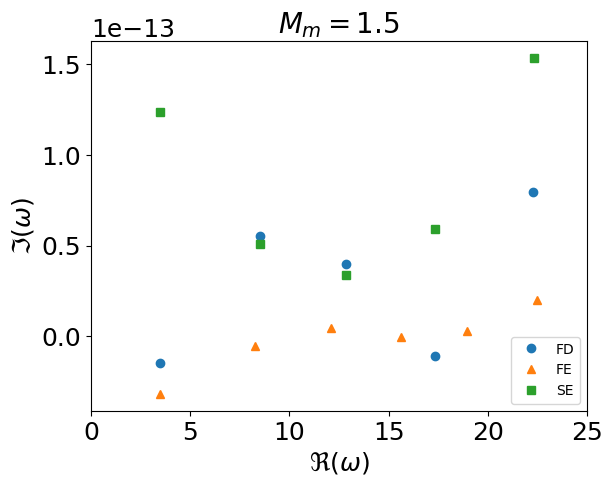
\includegraphics[width=0.7\linewidth]{figures/fixed-fixed-supersonic-v}
	\caption{First few filtered eigenvalues are shown. The spurious modes are filtered by convergence test.}
	\label{fig:supersonic-v-dirichlet}
\end{figure}

\subsection{Fixed-Open Boundary}
\begin{figure} [H]
	\centering
	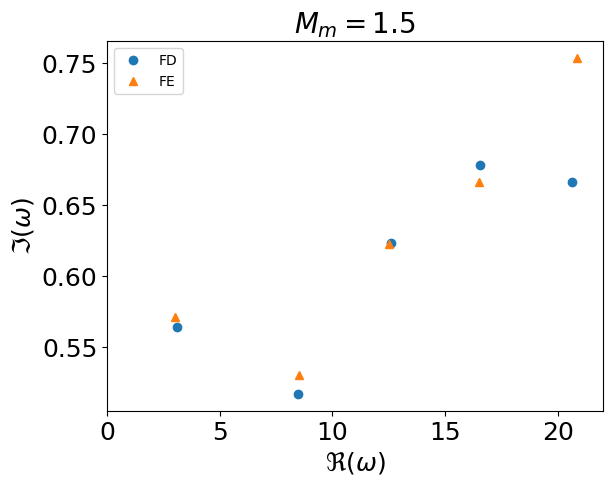
\includegraphics[width=0.7\linewidth]{figures/fixed-open-supersonic-v}
	\caption{All modes are unstable.}
	\label{fig:supersonic-v-fixed-open}
\end{figure}


\section{Accelerating Case}
Starting from the singular point, we shoot the solution to the left boundary. We find the set of eigenvalues such that $\tilde{v}(-1)=0$. With these eigenvalues, we can extend the solution to the supersonic region $(0,1]$. The first few eigenmodes are drawn in Fig.\ref{fig:results-accelerating-v}.
\begin{figure} [H]
	\centering
	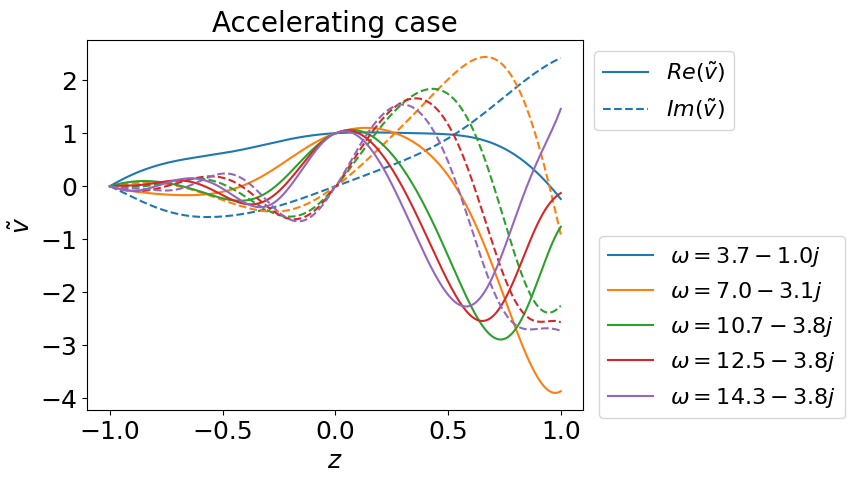
\includegraphics[width=0.7\linewidth]{figures/results-accelerating-v}
	\caption{The eigenmodes are stable.}
	\label{fig:results-accelerating-v}
\end{figure}

\section{Decelerating Case}
Again, we set the perturbations at the entrance of the nozzle to 0, $\tilde{v}(-1)=0$. Then we apply the same procedure as accelerating case, we obtained the following Fig.\ref{fig:results-decelerating-v}. The results indicates that the decelerating case is physically impossible with the selected boundary condition.
\begin{figure} [H]
	\centering
	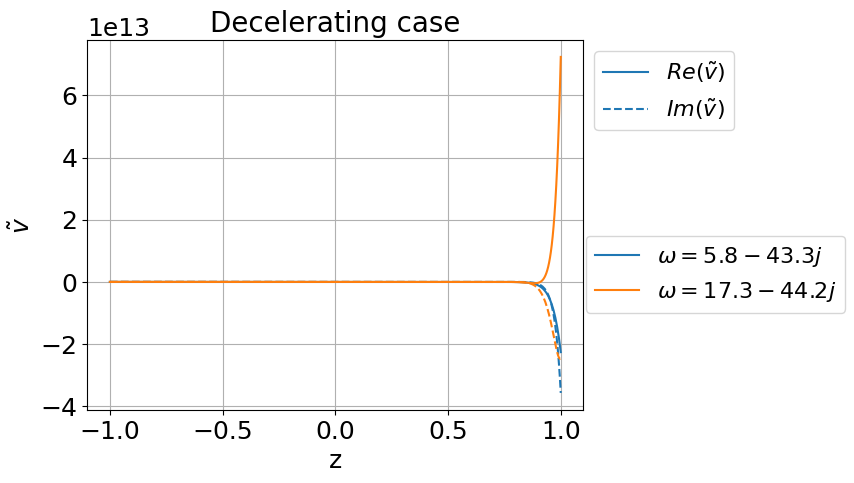
\includegraphics[width=0.7\linewidth]{figures/results-decelerating-v}
	\caption{The perturbations at the exit of the nozzle explode. It is not physically possible, therefore the decelerating case might not be physically with the given boundary condition.}
	\label{fig:results-decelerating-v}
\end{figure}

\chapter{Discussion} \label{chap:discussion}
\section{Summary of the Results}
In the first chapter we introduced various concepts including plasma, spectral instability and magnetic nozzle. We also briefly discussed the general procedure for finding the spectral instability of PDEs, and the relationship between spectral instability and plasma instability. In Chap.~\ref{chap:fluid-equations}, we derived the governing fluid equations for plasma flow in a magnetic nozzle and explored the equilibrium plasma flow. Following that, in Chap.~\ref{chap:polynomial-eigenvalue-problem}, by reducing the system of two first-order PDEs into a single second-order PDE, the problem simplifies to a so-called polynomial eigenvalue problem. In Chap.~\ref{chap:spectral-method} we discretized the Eq.~(\ref{eq:polynomial-eigenvalue-problem}) using Chebyshev differentiation matrix and Legendre polynomials, converting the polynomial eigenvalue problem into an algebraic eigenvalue problem. This allows us to apply well-developed numerical methods for obtaining eigenvalues and eigenfunctions. During this process, convergence test was applied to eliminate the spurious modes from spectral pollution. While spectral methods can handle most cases, i.e. subsonic and supersonic plasma flows, they fail to resolve meaningful eigenvalues and eigenfunctions for the accelerating plasma flow due to the existence of singularity at the sonic point in the nozzle throat. In Chap.~\ref{chap:singular-perturbation}, we addressed this issue. Frobenius method was used to pick up regular solutions passing through the nozzle throat and shooting method was applied on the regular solutions to find the eigenvalues and eigenfunctions.

For the subsonic flow, it is stable under Dirichlet boundary condition. It is also stable under fixed-open boundary, except for ground mode when velocity is nonuniform. For the supersonic flow, it is stable when Dirichlet boundary condition is applied, and unstable is the boundary condition is fixed-open. The flow with accelerating velocity profile is stable, assuming there is no velocity perturbation at the entrance of the nozzle. The results are summarized below.

\begin{itemize}
	\item Subsonic plasma flow is stable under Dirichlet boundary and is also stable (except ground mode with non-constant velocity profile) under Fixed-Open boundary.
	\item Supersonic plasma flow is stable under Dirichlet boundary but unstable under fixed-open boundary condition.
	\item Accelerating plasma flow is stable with Dirichlet boundary at the entrance.
\end{itemize}

\section{Limitations and Future Works}
\subsection{Spectral Method}
The spectral method suffers the spectral pollution. For now there is no automatic ways to filter spurious modes other than doing convergence test and pick up the convergent eigenvalues manually by ourselves. We believe there is a discretization scheme that is spectral pollution free. We made such optimistic guess based on the following example. Let's transform Eq.~\ref{eq:constant-v-problem-dirichlet} with Dirichlet boundary condition $\tilde{v}(\pm 1) = 0$ to its normal form, that is
\begin{equation}
	u''(z) + r(z)u(z) = 0, \quad u(\pm 1) = 0
\end{equation}
by doing the change of variables
\begin{equation}
	u(z) = \exp\left(\frac{iv_0\omega}{1-v_0^2}\right)\tilde{v}(z); \quad
	r(z) = \frac{\omega^2}{(1-v_0^2)^2}
\end{equation}
If we apply spectral methods to this problem, we observed no spurious modes in the spectrum. Meaning that this transformed problem is spectral pollution free. We might be able to transform the polynomial eigenvalue problem, with non-uniform velocity profile, to a certain form such that it is spectral pollution free when we apply spectral methods.

\subsection{Shooting Method}
The shooting method is not exhaustive due to the nature of root finding algorithm. A root can only be found if the initial guess of the root is close enough to the actual root. To work around this issue, we have to perform a grid search on the complex plane. This way we can only survey the low frequency region due to finite computing resources. The conclusion for the instability of accelerating plasma flow is true only for low frequency region. We believe there are different discretizations allowing us to overcome the singularity without picking up regular solutions manually using Frobenius method.



\bibliographystyle{plain}
\bibliography{references}
\nocite{*}
\appendix
% \chapter{Lambert $W$ Function} \label{app:lambert-w}
\begin{definition}
    The Lambert $W$ function is a function, $y(x)$, such that the following equation holds
    \[ ye^y = x \]
    where $y$ and $x$ are real. The Lambert $W$ function is denoted as $W_k(x)$, where $k=0,-1$ are its two branches.
\end{definition}
\begin{figure} [htbp]
    \centering
    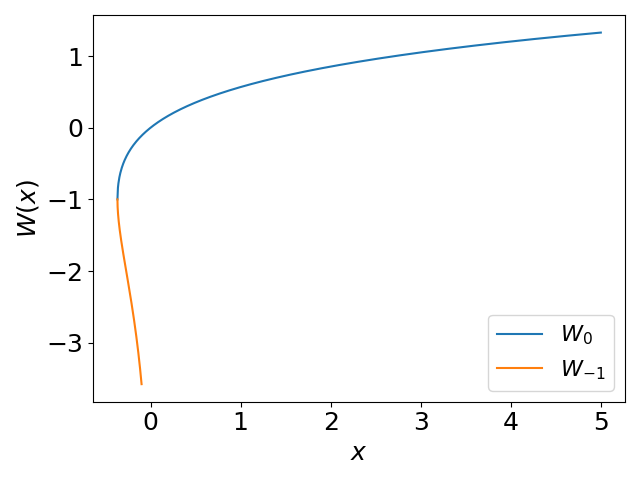
\includegraphics[width=0.7\textwidth]{figures/lambert-w.png}
    \caption{The graph of $y=W(x)$ for real $x<6$ and $y>-4$. The upper branch (blue) with $y\geq-1$ is the graph of the function $W_0(x)$ (principal branch), the lower branch (magenta) with $y\leq -1$ is the graph of the function $W_{-1}(x)$. The minimum value of $x$ is at $(-1/e,-1)$.}
    \label{fig:lambert-w}
\end{figure}
\chapter{Verification of Analytical Solutions}
The general solution to
\[
    \omega^2\tilde{v} + 2i\omega\pdv{\tilde{v}}{z} + (1-v_0^2)\pdv[2]{\tilde{v}}{z} = 0
\]
is
\[
    \tilde{v} = \exp(-\frac{i\omega}{v_0+1})
    \left[ \exp(i\omega\frac{z+1}{v_0+1})
        - \exp(i\omega\frac{z+1}{v_0-1}) \right]
\]
To show this, we first find the derivatives of $\tilde{v}$,
\begin{align*}
    \tilde{v}             & = \exp(-\frac{i\omega}{v_0+1})
    \left[ \exp(i\omega\frac{z+1}{v_0+1})
    - \exp(i\omega\frac{z+1}{v_0-1}) \right]                                                                     \\
    \pdv{\tilde{v}}{z}    & = i\omega\exp(-\frac{i\omega}{v_0+1})
    \left[ \frac{1}{v_0+1}\exp(i\omega\frac{z+1}{v_0+1}) - \frac{1}{v_0-1}\exp(i\omega\frac{z+1}{v_0-1}) \right] \\
    \pdv[2]{\tilde{v}}{z} & = -\omega^2\exp(-\frac{i\omega}{v_0+1})
    \left[ \frac{1}{(v_0+1)^2}\exp(i\omega\frac{z+1}{v_0+1}) - \frac{1}{(v_0-1)^2}\exp(i\omega\frac{z+1}{v_0-1}) \right]
\end{align*}
Then the rest is easy,
\begin{align*}
      & \omega^2\tilde{v} + 2i\omega\pdv{\tilde{v}}{z} + (1-v_0^2)\pdv[2]{\tilde{v}}{z}                                            \\
    = & \exp(-\frac{i\omega}{v_0+1})
    \left(1-\frac{2v_0}{v_0+1} + \frac{(1-v_0^2)}{(v_0+1)^2}\right)\exp(i\omega\frac{z+1}{v_0+1})
    \\
      & -\exp(-\frac{i\omega}{v_0+1})\left(1-\frac{2v_0}{v_0-1} + \frac{(1-v_0^2)}{(v_0-1)^2}\right)\exp(i\omega\frac{z+1}{v_0-1}) \\
    \\
    = & 0
\end{align*}

If $\omega = n\pi(1-v_0^2)/2$, then $\tilde{v}(\pm 1) = 0$.
It is easy to see that $v(-1)=0$. As for $z=1$, we have
\begin{align*}
    \tilde{v}(1) & \propto
    \exp(\frac{2i\omega}{v_0+1}) - \exp(\frac{2i\omega}{v_0-1}) \\
                 & =
    \exp(in\pi(1-v_0)) - \exp(-in\pi(1+v_0))                    \\
                 & =
    (-1)^n\exp(-in\pi v_0) - (-1)^n\exp(-in\pi v_0)             \\
                 & = 0
\end{align*}

If
\[\omega = (v_0^2-1) \left[ \frac{n\pi}{2} - \frac{1}{4}i\ln\left(\frac{v_0-1}{v_0+1}\right) \right]\]
then $\tilde{v}(-1) = 0$ and $\partial_z\tilde{v}(1) = 0$.
It is easy to see that $v(-1)=0$. The derivative at $z=1$ is
\begin{align*}
    \eval{\pdv{\tilde{v}}{z}}_{z=1} \propto &
    \frac{1}{v_0+1}\exp(\frac{2i\omega}{v_0+1}) - \frac{1}{v_0-1}\exp(\frac{2i\omega}{v_0-1})                                   \\
    =                                       & \frac{1}{v_0+1}\exp(in\pi(v_0-1) + \frac{v_0-1}{2}\ln(\frac{v_0-1}{v_0+1}))       \\
                                            & - \frac{1}{v_0-1}\exp(in\pi(v_0+1) + \frac{v_0+1}{2}\ln(\frac{v_0-1}{v_0+1}))     \\
    =                                       & \frac{(-1)^n}{v_0+1}\exp(in\pi v_0)\left(\frac{v_0-1}{v_0+1}\right)^{(v_0-1)/2}   \\
                                            & - \frac{(-1)^n}{v_0-1}\exp(in\pi v_0)\left(\frac{v_0-1}{v_0+1}\right)^{(v_0+1)/2} \\
    =                                       & 0
\end{align*}
The last equality holds because
\[ \frac{1}{v_0-1}\left(\frac{v_0-1}{v_0+1}\right)^{(v_0+1)/2}
    = \frac{1}{v_0+1}\left(\frac{v_0-1}{v_0+1}\right)^{(v_0-1)/2}  \]

\end{document}
